% Derivato dal mio template vecchio e da https://www.overleaf.com/latex/templates/template-tesi-universita-di-pisa/xwjmznxbtszd
%   Il progetto nasce dal template per il frontespizio realizzato da Marco Antonio Corallo, che ringrazio. Seguono alcuni commenti per evidenziare la presenza di alcuni pacchetti che mi sono stati utili per la stesura della tesi. Chiaramente, dipende tutto dal tipo di lavoro che uno vuole eseguire, che determina anche le diverse esigenze. Durante la stesura ho passato molto tempo su siti e forum a cercare di risolvere alcuni probelmi di formattazione, ma in generale Latex è stato piuttosto versatile. 

% Tipo di documento. L'uso di twoside implica che i capitoli inizino sempre con la prima pagina a sinistra, eventualmente lasciando una pagina vuota nel capitolo precedente. Se questa cosa è fastidiosa, è possibile rimuoverlo. 
\documentclass[a4paper]{report}

% Dimensione dei margini
\usepackage[a4paper,top=3cm,bottom=3cm,left=3cm,right=3cm]{geometry} 
% Dimensione del font
\usepackage[fontsize=13pt]{scrextend}
% Lingua del testo
\usepackage[english]{babel}
% Lingua per la bibliografia
\usepackage[fixlanguage]{babelbib}
% Codifica del testo
\usepackage[utf8]{inputenc} 
% Encoding del testo
\usepackage[T1]{fontenc}
% Permette di generare testo fittizio.
\usepackage{lipsum}
% Per ruotare le immagini
\usepackage{rotating}
% Per modificare l'header delle pagine 
\usepackage{fancyhdr}           

\usepackage{float}
\usepackage{caption}
\usepackage{subcaption}

% Librerie matematiche
\usepackage{amssymb}
\usepackage{amsmath}
\usepackage{amsthm}         

% Uso delle immagini
\usepackage{graphicx}
% Uso dei colori
\usepackage[dvipsnames]{xcolor}         
% Uso dei listing per il codice
\usepackage{listings}          
% Per inserire gli hyperlinks tra i vari elementi del testo 
\usepackage{hyperref}     
% Diversi tipi di sottolineature
\usepackage[normalem]{ulem}

\usepackage{tikz}

\usepackage[ruled,vlined]{algorithm2e}
\usepackage{algorithmic}
\usepackage{booktabs}
\usepackage{comment}
\usepackage[super]{nth}
\usepackage{booktabs}

% -----------------------------------------------------------------

% Modifica lo stile dell'header
\pagestyle{fancy}
\fancyhf{}
\lhead{\rightmark}
\rhead{\textbf{\thepage}}
\fancyfoot{}
\setlength{\headheight}{12.5pt}

% Rimuove il numero di pagina all'inizio dei capitoli
\fancypagestyle{plain}{
  \fancyfoot{}
  \fancyhead{}
  \renewcommand{\headrulewidth}{0pt}
}

\newcommand\independent{\protect\mathpalette{\protect\independenT}{\perp}}
\def\independenT#1#2{\mathrel{\rlap{$#1#2$}\mkern2mu{#1#2}}}

% Stile del codice
\lstdefinestyle{codeStyle}{
    % Colore dei commenti
    commentstyle=\color{teal},
    % Colore delle keyword
    keywordstyle=\color{Magenta},
    % Stile dei numeri di riga
    numberstyle=\tiny\color{gray},
    % Colore delle stringhe
    stringstyle=\color{violet},
    % Dimensione e stile del testo
    basicstyle=\ttfamily\footnotesize,
    % newline solo ai whitespaces
    breakatwhitespace=false,     
    % newline si/no
    breaklines=true,                 
    % Posizione della caption, top/bottom 
    captionpos=b,                    
    % Mantiene gli spazi nel codice, utile per l'indentazione
    keepspaces=true,                 
    % Dove visualizzare i numeri di linea
    numbers=left,                    
    % Distanza tra i numeri di linea
    numbersep=5pt,                  
    % Mostra gli spazi bianchi o meno
    showspaces=false,                
    % Mostra gli spazi bianchi nelle stringhe
    showstringspaces=false,
    % Mostra i tab
    showtabs=false,
    % Dimensione dei tab
    tabsize=2
} \lstset{style=codeStyle}

% Stile di codice per dimensioni maggiori, in cui ho avuto bisogno di un testo più picolo (ad esempio se si vuole inserire del codice che ha linee molto lunghe). Per usare questo stile piuttosto che il precedente, usare 

% \lstset{style=longBlock}
%  % inserire il codice...
% \lstset{style=codeStyle}

% Il secondo comando consente di tornare allo stile precedente 
\lstdefinestyle{longBlock}{
    commentstyle=\color{teal},
    keywordstyle=\color{Magenta},
    numberstyle=\tiny\color{gray},
    stringstyle=\color{violet},
    basicstyle=\ttfamily\scriptsize,
    breakatwhitespace=false,         
    breaklines=true,                 
    captionpos=b,                    
    keepspaces=true,                 
    numbers=left,                    
    numbersep=5pt,                  
    showspaces=false,                
    showstringspaces=false,
    showtabs=false,                  
    tabsize=2
} \lstset{style=codeStyle}

% Togliendo il commento al comando che segue, si inseriscono nella bibliografia anche le fonti presenti in Bibliography.bib ma non citati direttamente con il comando \cite
% \nocite{*}

% Margini prima e dopo blocchi di codice, per avere più distanza
\lstset{aboveskip=20pt,belowskip=20pt}

% Aggiunti definizioni, teoremi, linea e listing
\newtheorem{definition}{Definition}[section]
\newtheorem{theorem}{Theorem}[section]
\providecommand*\definitionautorefname{Definition}
\providecommand*\theoremautorefname{Theorem}
\providecommand*{\listingautorefname}{Listing}
\providecommand*\lstnumberautorefname{Line}

\raggedbottom

%\newcommand{\cgs}[1]{{\textcolor{brown}[\textcolor{red}{\bf{GS: }}{ \textcolor{brown}{#1]}}}}             
%\newcommand{\cmc}[1]{{\textcolor{blue}[\textcolor{magenta}{\bf{MC: }}{ \textcolor{blue}{#1]}}}}


% -----------------------------------------------------------------
\begin{document}

\include{chapters/Frontespizio}

\chapter*{Abstract}

\section*{English Version}


\section*{Versione Italiana}

\tableofcontents

% Rimuovere se non si vuole la tabella delle figure
\listoffigures

\chapter{Introduction}

\section{Data Scarcity and Noisy Datasets in Machine Learning}

\textbf{Machine Learning} (ML) is reshaping our world in ways both
subtle and profound. From the personalized recommendations we receive
on streaming platforms to the autonomous vehicles navigating in real streets,
ML algorithms are becoming an integral part of our daily lives.
Yet, as these systems tackle increasingly complex challenges,
they reveal their limitations.
One of the most pressing issues is the critical need for large, 
high-quality datasets, a requirement that is often difficult to
meet in real-world scenarios.

The \textbf{scarcity} of comprehensive datasets poses a significant
obstacle in many fields, including healthcare and robotics.
In \textbf{healthcare}, privacy concerns and limited access to patient
records hinder the collection of diverse and extensive data.
Similarly, in \textbf{robotics}, certain experimental data may be difficult
or costly to obtain, particularly in scenarios involving complex
physical interactions or rare events. This data scarcity can lead
to underfitted or non-generalizable models, compromising their
accuracy and utility in practical applications.

Moreover, even when substantial datasets are available, they
often suffer from \textbf{noise and inconsistencies}. Real-world data
collection processes are rarely perfect, resulting in datasets
that may contain outliers or biased samples, also due to unmeasured
variables and confounding factors.
These imperfections can significantly impact the performance of ML models,
leading to unreliable predictions or decisions. The challenge of dealing
with noisy datasets is particularly acute in offline
\textbf{Deep Reinforcement Learning} (DRL) scenarios, where agents must learn
optimal policies from pre-collected experiences without the ability
to interact further with the environment.

To address these challenges, researchers have long employed
\textbf{data augmentation techniques}. Traditional data augmentation
methods involve
applying various transformations to existing data points to artificially
expand the dataset. In image processing, for instance, this might involve
rotations, flips, or color adjustments. While these techniques have proven
effective in many applications, they have limitations.
Notably, not all transformations produce valid or realistic data points,
especially in domains with complex underlying structures or causal relationships.

This is where the integration of \textbf{Causal Inference} into
ML frameworks offers a
promising solution. Causal inference focuses on understanding the
cause-and-effect relationships between variables, rather
than merely identifying correlations. By leveraging causal inference,
we can develop more sophisticated data augmentation techniques that
respect the underlying causal structure of the data-generating process.

In this thesis, we propose novel approaches to address the
challenges of data scarcity and noisy datasets by leveraging
causal inference techniques. We introduce two frameworks for
counterfactual data generation:
the \textbf{Wasserstein Reward-enhanced CounTerfactual Data Generation}
(WRe-CTDG) and the \textbf{Supervised CounTerfactual Data Generation} (S-CTDG).
These methods aim to augment pre-collected datasets by generating additional
high-fidelity experiences that align with the environment's underlying
transition dynamics.

Our work focuses specifically on offline DRL scenarios, where agents
are trained using pre-collected datasets of experiences,
and we are going to explore applications in both robotics environments
and healthcare scenarios.

By incorporating \textbf{Structural Causal Models} (SCMs) and
\textbf{Generative Adversarial Networks} (GANs) into our frameworks,
we develop techniques to infer causal relationships and generate counterfactual
samples. This approach allows us to create synthetic data points
that are not mere transformations of existing data, but rather plausible
alternative scenarios that could have occurred under different circumstances.
This is particularly valuable in offline DRL, where the ability to explore
``what-if'' scenarios can significantly enhance the robustness
and generalization capabilities of learned policies.

\section{Thesis Overview}

The following chapters are organized as follows:
\begin{itemize}
    \item In \textbf{Chapter 2}, we provide an overview of the State of the Art
    in Offline Reinforcement Learning, Data Augmentation and Generation Techniques,
    and Counterfactual Reasoning in Data Generation.
    \item In \textbf{Chapter 3}, we introduce the theoretical foundations
    of the tecnologies used in our proposed frameworks,
    including Structural Causal Models,
    Generative Adversarial Networks,
    and Deep Reinforcement Learning algorithms.
    \item In \textbf{Chapter 4}, we present the WRe-CTDG
    and the S-CTDG frameworks,
    detailing their architectures and training procedures.
    We also present the environments and datasets used for evaluation.
    \item In \textbf{Chapter 5}, we present a description
    of the machines specifications
    and of the details of the neural networks employed in our experiments,
    followed by a detailed overview of the experimental results.
    \item In \textbf{Chapter 6}, we discuss the implications of our findings,
    the limitations of our approaches,
    and potential directions for future research.
\end{itemize}

\chapter{State of the Art}

\section{Offline RL: Advancements and Challenges}

\textbf{Offline Reinforcement Learning} (Offline RL)
has emerged as a promising approach for training control
policies using pre-collected experiences,
eliminating the need for potentially dangerous or
costly online interactions. Despite significant progress
in this field, several challenges persist in
its practical application, particularly in control
and robotics domains.

Research efforts to enhance Offline RL performance are
primarily advancing along two paths that we
are now going to explore.

\subsection{Improving Robustness and Sample Efficiency}

The first research direction focuses on refining
existing methods to enhance their robustness and
sample efficiency. \cite{kumar2021} propose a comprehensive
workflow for offline model-free robotic reinforcement
learning. Their approach addresses challenges specific
to real-world robotics applications, proposing
metrics and protocols to assist practitioners in
selecting policy checkpoints, regularization parameters,
and model architecture.

\cite{ijcai2023} introduce a hierarchical approach called
``Guide to Control'' that solves efficiently long-horizon
and sparse-reward tasks from offline data.
This method enhances the effectiveness
of offline RL in complex environments by breaking down the overall
task into more manageable sub-tasks, thereby improving learning
efficiency and performance.

\subsection{Developing Datasets and Benchmarks}

The second path concentrates on creating extensive datasets
and benchmarks tailored for control and robotics domains.
\cite{gurtler2023} present a benchmark for offline RL
on real-robot hardware, providing an useful resource for
evaluating algorithms in practical settings.
In their work they propose a set of
benchmark datasets for robotic manipulation
that are intended to help improving the
state-of-the-art in offline reinforcement learning.

\cite{liu2023} contribute datasets and benchmarks
specifically designed for offline safe reinforcement learning
to accelerate research in this area.
Their work addresses the critical aspect of safety in robotic
applications, providing resources for researchers to develop and
test algorithms that not only optimize performance but also ensure
safe operation in various scenarios. The suite comprises three
main components: expertly crafted safe policies, D4RL-styled
datasets with environment wrappers, and high-quality offline
safe RL baseline implementations. The authors present a methodical
data collection pipeline using advanced safe RL algorithms to generate
diverse datasets across 38 popular safe RL tasks,
ranging from robot control to autonomous driving.
They also introduce data post-processing filters to
modify dataset diversity, simulating various data collection conditions.

\section{Data Augmentation Strategies in RL}

Despite ongoing improvements in learning algorithms,
the quantity of training data continues to be a critical
determinant of success in machine learning processes.
This is especially challenging when dealing with complex,
high-dimensional inputs such as images, where the data requirements
for effective training are substantial.

To address the problem of limited data availability,
researchers and practitioners often turn to
\textbf{data augmentation techniques}.
These methods aim to expand existing datasets by generating
synthetic samples that are both artificial and plausible,
thereby enriching the training set without the need
for additional real-world data collection.

\cite{mumini2022} provide a comprehensive survey of modern data
augmentation approaches, highlighting their potential in
enhancing computer vision across various domains.

\subsection{Augmentation in Online and Offline RL}

Both online and offline RL approaches have incorporated data
augmentation techniques to improve learning efficiency and generalization.

In the \textbf{online} RL setting, \cite{laskin2020}
introduce Reinforcement Learning with Augmented Data (RAD), 
a simple module designed to enhance most RL algorithms.
The authors conduct an extensive study of various data augmentation
techniques for both pixel-based and state-based inputs in RL, including
two new augmentations they introduce: random translate and random
amplitude scale.

\cite{hansen2021} further further explore the concept of data augmentation
in online RL, proposing SOft Data Augmentation (SODA),
a novel approach to improve generalization in RL;
unlike traditional methods that directly learn policies
from augmented data, SODA decouples augmentation from policy learning.
It does this by applying a soft constraint on the encoder to
maximize mutual information between latent representations of
augmented and non-augmented data, while using only non-augmented
data for RL optimization.

In the \textbf{offline} RL setting, \cite{han2022}
introduce a selective data augmentation technique
using a Variational Autoencoder.

A \textbf{Variational Autoencoder} (VAE),
defined in \cite{kingma2013},
is an unsupervised learning architecture
that learns a low-dimensional latent space
representation of the input data
by encoding and decoding it through
two separate neural networks.
\label{sec:vae}

The method of \cite{han2022} targets sparse subspaces in the dataset,
representing them in the VAE's latent space,
then sampling and decoding new data points to augment
underrepresented regions. This approach aims to generate
virtual data that closely aligns with the original data distribution.

\cite{joo2022} propose a data augmentation method for offline RL
called Swapping Target Q-Value (SQV).
SQV works by swapping Q-values between original and transformed images,
encouraging the algorithm to treat similar states as equivalent while
emphasizing differences between distinct states.
This method aims to enhance pixel-based learning without auxiliary
loss functions, potentially improving performance and generalization
in offline RL scenarios with limited datasets.

\subsection{Dynamics-Aware Augmentation}

Traditional augmentation methods often operate without
knowledge of the underlying environment dynamics, requiring
careful tuning to avoid generating inconsistent samples.
To mitigate this issue, dynamics-aware augmentation schemes
have emerged in the robotics field.

In a paper by \cite{lin2020} the authors introduce a
framework called
\textbf{Invariant Transform Experience Replay}
to improve Deep Reinforcement Learning (DRL)
for robot control.
The main idea is to use symmetries in robotic
tasks to create more training data by exploiting
reflectional symmetries and taking advantage of
flexible goal definitions.

Nonetheless, effectively implementing these techniques
requires an in-depth understanding
of the underlying process, which is often not available, and
the development of an augmentation strategy specifically
crafted for the task at hand.

\section{Learning-Based Approaches to Data Generation}

Researchers are increasingly turning to data-driven methods
to overcome these obstacles. These approaches aim to learn
the underlying data generation model from the offline
dataset itself. After the model is trained,
it can be used to produce new samples that align
with the environment's dynamics. This strategy allows
for the creation of synthetic data that is more likely
to be consistent with the real-world processes
being modeled, without requiring explicit knowledge
of those processes.

\subsection{Transformer-Based Models}

\cite{wang2022} introduce the Bootstrapped Transformer,
a novel algorithm for offline RL.
They approach offline RL as a sequence generation
problem, using \textbf{Transformer} models to represent
trajectories. Recognizing the common issue of
limited and insufficiently diverse training
data in offline RL datasets, they implement a
\textbf{bootstrapping technique}: 
this allows the model to generate additional
offline data using its own learned representations,
which is then used to enhance the training of
the sequence model.

\subsection{World Models and Variational Autoencoders}

\textbf{World Models}, introduced in \cite{ha2018},
are a class of models that combine a Variational
Autoencoder as a Vision module,
a Recurrent Neural Network (RNN)
with a Mixture Density Network (MDN) as a Memory
module and a simple Neural Network (NN)
layer as a Controller.
These models can be trained
quickly in an unsupervised manner to learn a
compressed spatial and temporal representation
of the environment.

Despite not being explicitly designed for data augmentation,
World Models and VAEs
can be naturally used to achieve the same objective.

\cite{hafner2020} 
introduces \textbf{Dreamer}, a reinforcement learning
agent that uses a learned world model to solve complex
tasks from visual inputs. Dreamer learns a compact
latent space representation of the environment and
uses this model to imagine trajectories and learn
behaviors through ``latent imagination''.
The agent learns both actions and state values in the
latent space, efficiently optimizing behavior
by propagating analytic gradients of learned
state values through imagined trajectories.

A similar approach was proposed in \cite{andersen2018},
where the \textbf{Dreaming Variational Autoencoder} (DVAE)
architecture is presented.
The DVAE combines variational autoencoders
with deep reinforcement learning agents,
allowing agents to learn optimal policies using
generated training data samples. To test this approach,
the authors also present \textbf{Deep Maze}, a novel and flexible
maze engine that provides various challenges
for reinforcement learning algorithms,
including partial and fully-observable state-spaces,
long-horizon tasks, and both deterministic and
stochastic problems.

\section{Counterfactual Reasoning in Data Generation}

The \textbf{counterfactual-based approach} offers a
versatile and robust alternative rooted in
the theory of \textbf{Structural Causal Models} (SCMs) 
(which are discussed in more detail in Section
\ref{sec:scm}).
This method begins by modeling the system's
dynamics using an SCM, which is then employed
for counterfactual reasoning. This process generates
new samples as counterfactual outcomes that align with
the model. Unlike previous methods, SCMs provide
tools to model and estimate unmeasured variables,
enabling a more precise depiction of the factors
affecting the system's behavior.

\subsection{Counterfactual Generative Models}

\cite{sauer2021} introduce the
\textbf{Counterfactual Generative Network} (CGN),
a novel approach to improve the robustness and
interpretability of image classifiers.
The authors propose decomposing the image
generation process into independent causal
mechanisms that disentangle object shape, texture
and background. This allows for the generation of
counterfactual images, synthetic images with novel
combinations of these features.
The CGN is trained without direct supervision,
using only class labels and inductive biases and
the authors demonstrate the CGN's ability to
generate counterfactual images
on MNIST and ImageNet datasets, as shown
in Figure \ref{fig:ctf}.

\begin{figure}[ht]
    \centering
    \includegraphics[width=\textwidth]{figures/ch2/1.ctf2.png}
    \caption{ImageNet Counterfactuals produced by the CGN}
    \vspace{-10px}
    \caption*{\scriptsize{Source: \cite{sauer2021}}}
    \label{fig:ctf}
\end{figure}

Another usage of counterfactual reasoning,
this time in the context of medical imaging,
is presented in \cite{mertes2022}.
This paper introduces GANterfactual,
a novel approach for generating counterfactual
explanations for image classifiers using adversarial
image-to-image translation techniques.
Unlike traditional methods that highlight
important areas in images, GANterfactual
modifies input images to change the
classifier's prediction,
providing users with a different kind
of explanatory information.
The authors focus on medical contexts,
specifically pneumonia detection in chest X-rays,
where textural and structural information is necessary.

\subsection{Counterfactual Data Augmentation in Offline RL}

\cite{lu2020} investigate counterfactual-based
data augmentation
specifically in the context of Offline RL.
They propose a Deep Generative Model based on the
Bidirectional Conditional Generative Adversarial Network
(BiCoGAN) architecture (which is discussed in more detail
in Section \ref{sec:bicogan}), the model
can be seen in Figure \ref{fig:rlcf}.
The authors use SCMs
to model state dynamics, leveraging both
commonalities and differences across subjects,
and allowing to estimate unmeasured variables,
which are then used to effectively
reproduce the environment’s initial conditions
and enable the
generation of counterfactual outcome.
They prove that counterfactual outcomes are identifiable
under mild conditions and that a Double Dueling
Deep Q-Network (discussed in Section \ref{sec:rl})
trained on both the augmented dataset and the original
counterpart achieves better performance on the first one.

\begin{figure}[h]
    \centering
    \includegraphics[width=.5\textwidth]{figures/ch2/2.rlcf.png}
    \caption{The proposed Deep Generative Model for Counterfactual Data Augmentation in Offline RL}
    \vspace{-10px}
    \caption*{\scriptsize{Source: \cite{lu2020}}}
    \label{fig:rlcf}
\end{figure}

However, this approach is designed for non-visual,
low-dimensional inputs, and discrete control
actions. Additionally, a significant drawback of this algorithm
is its lack of a mechanism for estimating the reward
associated with the generated states. This limitation implies
that retrieving the reward is possible only when the reward
function can be directly calculated from the generated states,
a condition that does not always apply.
 

\chapter{Theoretical Background}

\section{Deep Learning}
\label{sec:dl}

In the field of machine learning, the first models you
are often introduced to are those for regression
and classification that utilize linear
combinations of fixed basis functions.
According to \cite{Bishop:2008aa},
these models possess useful analytical and computational properties,
but their practical applicability is constrained 
since their capacity is limited to linear functions
and they cannot understand the interaction between any two input variables.
This leads to problems such as the \textbf{curse of dimensionality},
where the number of possible interactions between variables grows exponentially
with the number of input variables.
To address large-scale problems, it is essential to adapt the basis functions
to the data, as demonstrated by Support Vector Machines (SVMs).
Alternatively, one can fix the number of basis functions in advance while
allowing them to be adaptive, utilizing parametric forms for the basis
functions with parameter values adjusted during training.

The most successful example of this approach in pattern recognition is the
\textbf{feed-forward neural network},
also known as the \textbf{MultiLayer Perceptron} (MLP).
\begin{figure}[h]
    \centering
    \includegraphics[width=.75\textwidth]{figures/ch3/1.mlp.png}
    \caption{A feed-forward neural network with two hidden layers}
    \vspace{-10px}
    \caption*{\scriptsize{Source: \href{https://brilliant.org/wiki/feedforward-neural-networks/}{Brilliant}}}
    \label{fig:mlp}
\end{figure}

As explained in 
\cite{goodfellow2016deep},
the goal of a feedforward network is to approximate a specific function
\( f^* \). For example, in a classification task,
\( y = f^*(x) \) maps an input \( x \) to a category \( y \).
A feedforward network defines a mapping \( y = f(x; \theta) \) and
learns the parameters \( \theta \) that yield the best approximation
of this function.

These models are called \textbf{feedforward} because information
flows unidirectionally from the input \( x \), through intermediate computations
defining \( f \), and ultimately to the output \( y \), without feedback loops.

The training data directly specifies the behavior of the output layer but
not the intermediate layers, which are called \textbf{hidden layers}
since their desired outputs are not provided by the training data.
The learning algorithm must determine how to best utilize these
hidden layers to approximate \( f^* \).
Every layer of the network computes a non-linear transformation of the
previous layer's activations, this way a complex function can be
approximated by composing simpler functions, one for each layer.
Layers are composed of a set of \textbf{units}, where each unit is a node that
computes a non-linear function of the weighted sum of its inputs
and is only connected to units in the previous and the following layer.

In order to train the network and update the weights, MLPs use the
\textbf{backpropagation} technique, which computes the gradient of the
loss function with respect to the weights of the network.
The weights are then updated using an optimization algorithm such as
\textbf{Stochastic Gradient Descent} (SGD)
or one of its adaptive variants like \textbf{Adam},
whose hyperparameters are tuned according to the task during training.

A feedforward network is called a \textbf{deep neural network} if it has
more than one hidden layer, the branch of machine learning that studies
deep neural networks is called \textbf{deep learning}.

They are called networks due to their structure, which involves composing
multiple functions together. Typically, this composition is represented
by a directed acyclic graph. For instance, functions
\( f^{(1)} \), \( f^{(2)} \), and \( f^{(3)} \) might be connected in
a chain to form \( f(x) = f^{(3)}(f^{(2)}(f^{(1)}(x))) \).

Functions \( f^{(1)} \) and \( f^{(2)} \) must
be non linear, otherwise the composition would collapse into a single
linear function. These non-linear functions are
called \textbf{activation functions}.
The last function \( f^{(3)} \) is typically a linear function that maps
the output of the final hidden layer to the output layer.
This is the same as applying a linear model to a transformed
input \( \phi(x) \), where \( \phi \) is a nonlinear transformation.
The question then becomes how to choose the mapping \( \phi \).

The strategy of deep learning is to learn \( \phi \):
in this approach, we use a model
\begin{equation}
y = f(x; \theta, w) = \phi(x; \theta)^\top w
\end{equation}
Here, we have parameters \( \theta \) that are used to learn \( \phi \)
from a broad class of functions, and parameters \( w \) that map \( \phi(x) \)
to the desired output.
This approach allows for greater flexibility:
specifically, by using a broad family of functions
\( \phi(x; \theta) \), the human designer only needs to select the appropriate
general function family rather than finding precisely an exact function.

The \textbf{universal approximation theorem} \cite{HORNIK1989359}
tells us that regardless of what function
we are trying to learn, we know that a feedforward network with enough units
will be able to \emph{represent} this
function, however we are not guaranteed that the training algorithm will be able
to \emph{learn} it.

\subsection{Convolutional Neural Networks}
\label{sec:cnn}

\textbf{Convolutional Neural Networks} (CNNs) are a specialized type of neural network
for processing data that has a known, grid-like topology,
it is particularly effective for image recognition tasks.

The key components of CNNs are:
\begin{itemize}
    \item \textbf{Convolutional layers}: These layers apply a convolution operation
    to the input, passing the result to the next layer.
    The input grid is convolved with a set of filters,
    also known as \textbf{kernels}, which are small windows that move across the input grid
    and apply a convolution operation between the input and the kernel weight
    at each position. The weight of the kernel is learned during training.
    Each convolutional layer applies multiple filters to the input, each producing
    a different \textbf{feature map}.
    \item \textbf{Pooling layers}: These layers downsample the feature maps
    produced by the convolutional layers to reduce the dimensionality of the data.
    This reduces the computational complexity of the network and helps to focus
    on the most important elements of the input.
    \item \textbf{Fully connected} (FC) \textbf{layers}: These layers connect every neuron
    in one layer to every neuron in another layer.
    It is in these layers that the features learned by the convolutional layers
    are used to classify the input image.
\end{itemize}
An example of a CNN classification architecture is shown in Figure \ref{fig:cnn}.

\begin{figure}[h]
    \centering
    \includegraphics[width=\textwidth]{figures/ch3/8.cnn.png}
    \caption{A typical CNN architecture for classification.}
    \vspace{-10px}
    \caption*{\scriptsize{Source: \href{https://towardsdatascience.com/a-comprehensive-guide-to-convolutional-neural-networks-the-eli5-way-3bd2b1164a53}{Sumit Saha}}}
    \label{fig:cnn}
\end{figure}

CNNs have been shown to achieve state-of-the-art performance on
a variety of computer vision tasks, including image classification,
object detection and image segmentation.
They have also been successfully applied to other types of data,
such as speech recognition and natural language processing.

\section{Reinformcement Learning}
\label{sec:rl}

``\textbf{Reinforcement learning} is learning [...] how
to map situations to actions so
as to maximize a numerical reward signal.
The learner is not told which actions to
take, but instead must discover which actions
yield the most reward by trying them. In
the most interesting and challenging cases, actions may
affect not only the immediate
reward but also the next situation and,
through that, all subsequent rewards.
These two
characteristics, \textbf{trial-and-error search} and \textbf{delayed reward},
are the two most important
distinguishing features of reinforcement learning.'' \cite{sutton1998}

Let's explore the basic concepts of reinforcement learning with
a simple example as described in \cite{zhao2024RLBook}.
Consider a grid world scenario as shown in Figure \ref{fig:rl}
where a robot, referred to as
the \textbf{agent}, moves between cells, occupying one cell at a time.
The white cells are accessible, while the orange cells are forbidden.
The goal is for the agent to reach a target cell.

\begin{figure}[h]
    \centering
    \includegraphics[width=.42\textwidth]{figures/ch3/2.rl.png}
    \caption{A simple reinforcement learning task}
    \vspace{-10px}
    \caption*{\scriptsize{Source: \cite{zhao2024RLBook}}}
    \label{fig:rl}
\end{figure}

To achieve this, the agent needs a \textbf{policy} that guides it to the target
efficiently, avoiding forbidden cells and unnecessary detours.
If the grid layout is known, planning is simple.
However, without prior knowledge, the agent must explore and learn
through trial and error.

The agent's status in the grid is defined by its \textbf{state}
\( s_i \in \mathcal{S} \), which represents its location relative
to the \textbf{environment}.
In the examples with nine cells, the state space is
\( \mathcal{S} = \{s_1, s_2, \ldots, s_9\} \)..

From each state, the agent can perform five \textbf{actions}: move up,
right, down, left or stay put, denoted as \( a_1, a_2, \ldots, a_5 \),
this set of actions is the action space
\( \mathcal{A} = \{a_1, \ldots, a_5\} \).
The available actions can vary by state, for instance,
at \( s_1 \), actions \( a_1 \) (up) and \( a_4 \) (left) would collide
with the grid boundary, so the action space is
\( \mathcal{A}(s_1) = \{a_2, a_3, a_5\} \).

When taking an action, the agent may move from one state to another,
a process known as \textbf{state transition}. For example,
if the agent is at state \( s_1 \) and selects action
\( a_2 \) (moving rightward), it transitions to state
\( s_2 \). This process can be represented as:
\[ s_1 \overset{a_2}{\longrightarrow} s_2 \]
The state transition process is defined for each
state and its associated actions. Mathematically, state transitions
are described by conditional probabilities.
For example, for \( s_1 \) and \( a_2 \),
the conditional probability distribution is:
\[
\begin{aligned}
p(s_1 \mid s_1, a_2) &= 0, \\
p(s_2 \mid s_1, a_2) &= 1, \\
p(s_3 \mid s_1, a_2) &= 0, \\
p(s_4 \mid s_1, a_2) &= 0, \\
p(s_5 \mid s_1, a_2) &= 0,
\end{aligned}
\]
indicating that taking \( a_2 \) at \( s_1 \) guarantees
the agent moves to \( s_2 \), with a probability of one,
and zero probability for other states.

This is a deterministic state transition,
but state transitions can also be stochastic,
requiring conditional probability distributions.
For instance, if random wind gusts affect the grid,
taking action \( a_2 \) at \( s_1 \) might blow the agent to \( s_5 \)
instead of \( s_2 \), resulting in \( p(s_5 \mid s_1, a_2) > 0 \).

A \textbf{policy} is a function that maps states to actions,
indicating the agent's behavior in the environment.
In other words, a policy tells the agent what action to take
at each state.

Mathematically, policies can be described by conditional probabilities.
For example, the policy for \( s_1 \) is:
\[
\begin{aligned}
\pi(a_1 \mid s_1) &= 0, \\
\pi(a_2 \mid s_1) &= 1, \\
\pi(a_3 \mid s_1) &= 0, \\
\pi(a_4 \mid s_1) &= 0, \\
\pi(a_5 \mid s_1) &= 0,
\end{aligned}
\]
indicating that the probability of taking action \( a_2 \) at state \( s_1 \)
is one, and the probabilities of taking other actions are zero.

The above policy is deterministic, but policies may generally be stochastic.
For instance, let's assume that at state \( s_1 \)
the agent may take actions to move either rightward or downward,
each with a probability of 0.5. In this case, the policy for \( s_1 \) is:
\[
\begin{aligned}
\pi(a_1 \mid s_1) &= 0, \\
\pi(a_2 \mid s_1) &= 0.5, \\
\pi(a_3 \mid s_1) &= 0.5, \\
\pi(a_4 \mid s_1) &= 0, \\
\pi(a_5 \mid s_1) &= 0.
\end{aligned}
\]

After executing an action at a state, the agent receives a
reward \( r \) as feedback from the environment.
The \textbf{reward} is a function of the state and action
which predicts immediate reward and is denoted as:
\begin{equation}
R(s_t=s, a_t=a) = \mathbb{E} [r_t | s_t = s, a_t = a]
\end{equation}
and it can be positive, negative, or zero.
Different rewards influence the policy the agent learns.
Generally, a positive reward encourages the agent to take the
corresponding action, while a negative reward discourages it.

However we can't find good policies
by simply selecting actions with the greatest immediate rewards
since they do not consider
long-term outcomes. To determine a good policy, we must consider the total
reward obtained in the long run and
an action with the highest immediate reward may not lead to
the greatest total reward.

A \textbf{trajectory} is a state-action-reward chain.
For example, the agent in our example may follow this trajectory:
\[ s_1 \xrightarrow{a_2, r=0} s_2 \xrightarrow{a_3, r=0} s_5 \xrightarrow{a_3, r=0} s_8 \xrightarrow{a_2, r=1} s_9. \]
The \textbf{return} of this trajectory is the sum of all rewards collected along it,
in the example above:
\[\text{return} = 0+0+0+1=1\]
Returns, also called total rewards or cumulative rewards,
are used to evaluate policies.
Returns can also be defined for infinitely long trajectories, which may diverge.
Therefore, we introduce the concept of \textbf{discounted return} for infinitely
long trajectories. The discounted return is the sum of the rewards from $t$ to $T$ (final step):
\begin{equation}
G_t \doteq R_{t+1} + \gamma R_{t+2} + \gamma^2 R_{t+3} + \ldots = \sum_{k=0}^{\infty} \gamma^k R_{t+k+1}
\end{equation}
where \( \gamma \in [0, 1] \) is the \textbf{discount factor}.
If \( \gamma \) is close to 0, the agent emphasizes near-future rewards,
resulting in a short-sighted policy. If \( \gamma \) is close to 1,
the agent emphasizes far-future rewards.

When $T$ is finite, we call the task episodic and each sequence
up to the \textbf{terminal state} is an \textbf{episode}. Otherwise, we refer
to \textbf{continuing tasks}.

The \textbf{Markov Decision Processes} (MDPs),
a general framework for describing stochastic dynamical systems,
allows us to formally presents these concepts.
The \textbf{Markov property} refers to the \textbf{memoryless} property of a stochastic process. Mathematically, it means that
\begin{equation}
\begin{aligned}
p(s_{t+1} \mid s_t, a_t, s_{t-1}, a_{t-1}, \ldots, s_0, a_0) &= p(s_{t+1} \mid s_t, a_t), \\
p(r_{t+1} \mid s_t, a_t, s_{t-1}, a_{t-1}, \ldots, s_0, a_0) &= p(r_{t+1} \mid s_t, a_t),
\end{aligned}
\end{equation}
where \( t \) represents the current time step and \( t + 1 \) represents the next time step.
This indicates that the next state or reward depends only on the current
state and action and is independent of the previous ones.

\vspace{3cm}

An MDP is defined by a tuple \( \langle \mathcal{S}, \mathcal{A}, P, R, \gamma \rangle \),
let us break down the components:
\begin{itemize}
    \item \( \mathcal{S} \): finite set of Markov states $s$
    \item \( \mathcal{A} \): finite set of actions $a$
    \item \( P \): state transition model for each action,
    a probability matrix that specifies $$p(s_t+1 = s'|s_t=s, a_t=a)$$
    \item \( R \): reward function
    $$ R(s_t=s, a_t=a) = \mathbb{E} [r_t | s_t = s, a_t = a] $$
    \item \( \gamma \): discount factor $0 \leq \gamma \leq 1$
\end{itemize}

When the policy in a MDP is fixed, it reduces to a \textbf{Markov Process} (MP),
this transformation simplifies the MDP by eliminating the decision-making aspect. 
A Markov process is referred to as a \textbf{Markov Chain} if it operates in discrete
time and the number of states is either finite or countable.

\begin{figure}[h]
    \centering
    \includegraphics[width=.75\textwidth]{figures/ch3/3.mdp.png}
    \caption{The example grid as a Markov Process graph, where the nodes
    represent the states and the edges represent the state transitions.}
    \vspace{-10px}
    \caption*{\scriptsize{Source: \cite{zhao2024RLBook}}}
    \label{fig:mdp}
\end{figure}


\subsection{Reinforcement Learning Algorithms}
\label{sec:rlalg}

In \cite{openaiPartKinds}, the landscape of algorithms in modern reinforcement
learning is explored.

The algorithms used in reinforcement learning almost always rely on
\textbf{value functions}.
The \textbf{value} is the expected return if the agent starts in
that state or state-action pair and then follows a specific policy indefinitely.

\vspace{5cm}

There are four primary value functions to consider:

\begin{itemize}
    \item \textbf{On-Policy Value Function, \( V^{\pi}(s) \)}: This function
    represents the expected return if the agent starts in state \( s \)
    and acts according to the policy \( \pi \):
    \begin{equation}
    V^{\pi}(s) = \mathbb{E}_{\tau \sim \pi} \left[ R(\tau) \mid s_0 = s \right]
    \end{equation}
    \item \textbf{On-Policy Action-Value Function, \( Q^{\pi}(s,a) \)}:
    This function gives the expected return if the agent starts in state \( s \),
    takes an arbitrary action \( a \), and then always follows the policy \( \pi \):
    \begin{equation}
    Q^{\pi}(s,a) = \mathbb{E}_{\tau \sim \pi} \left[ R(\tau) \mid s_0 = s, a_0 = a \right]
    \end{equation}
    \item \textbf{Optimal Value Function, \( V^*(s) \):} This function provides
    the expected return if the agent starts in state \( s \) and follows the
    optimal policy for the environment:
    \begin{equation}
    V^*(s) = \max_{\pi} \mathbb{E}_{\tau \sim \pi} \left[ R(\tau) \mid s_0 = s \right]
    \end{equation}
    \item \textbf{Optimal Action-Value Function, \( Q^*(s,a) \):} This function
    represents the expected return if the agent starts in state \( s \),
    takes an arbitrary action \( a \), and then follows the optimal policy for the environment:
    \begin{equation}
    Q^*(s,a) = \max_{\pi} \mathbb{E}_{\tau \sim \pi} \left[ R(\tau) \mid s_0 = s, a_0 = a \right]
    \end{equation}
\end{itemize}

Figure \ref{fig:mdp}
presents a partial taxonomy of the modern reinforcement learning algorithms.
One key distinction is whether the agent utilizes (or learns) a model of
the environment. A model, in this context, refers to a function that predicts
state transitions and rewards.

\begin{figure}[h]
    \centering
    \includegraphics[width=.8\textwidth]{figures/ch3/4.rlalg.png}
    \caption{Partial taxonomy of algorithms in modern RL.}
    \vspace{-10px}
    \caption*{\scriptsize{Source: \cite{openaiPartKinds}}}
    \label{fig:mdp}
\end{figure}

The primary advantage of having a model is that it enables the agent
to plan by predicting future states and rewards.
However, the major drawback is that an accurate model of the environment
is often unavailable to the agent.
Algorithms which use a model are known as \textbf{model-based} methods,
while those that do not are referred to as \textbf{model-free} methods.
Our focus will be on the latter.

Model-free methods can be categorized into two main approaches
for representing and training agents:
\begin{itemize}
    \item \textbf{Policy Optimization:} explicitly represents a policy
    as \( \pi_{\theta}(a \mid s) \) and optimizes the parameters \( \theta \)
    either directly via gradient ascent on the performance objective
    \( J(\pi_{\theta}) \) or indirectly by maximizing local approximations
    of \( J(\pi_{\theta}) \).
    Typically, this optimization is performed \textbf{on-policy},
    meaning that each update uses data collected while the agent is acting
    according to the most recent version of the policy.

    \item \textbf{Q-Learning:} involves learning an approximator
    \( Q_{\theta}(s,a) \) for the optimal action-value function \( Q^*(s,a) \).
    Unlike policy optimization, Q-learning is generally performed \textbf{off-policy},
    allowing updates to use data collected at any time during training,
    irrespective of the agent's policy at the time of data collection.
    The corresponding policy is derived from the relationship between
    \( Q^* \) and \( \pi^* \), where the actions taken by the Q-learning
    agent are determined by
    \begin{equation}
    a(s) = \arg \max_a Q_{\theta}(s,a)
    \end{equation}
    An example of a Q-learning algorithm is Deep Q-Network (\textbf{DQN}),
    which uses a deep neural network to approximate the optimal action-value
    function in environments with large state spaces \cite{dqn},
    and its variants such as Double DQN (\textbf{DDQN})
    \cite{ddqn} and
    Dueling Double DQN (\textbf{D3QN}) \cite{d3qn}.
    This family of algorithms is used in tasks with discrete action spaces.

\end{itemize}

There are also hybrid approaches that combine elements
of both policy optimization and Q-learning.
In this spectrum of algorithms we can find 
\textbf{actor-critic methods}, which consist of two components:
an \textbf{actor} that makes actions and a \textbf{critic} that evaluates them.
An example of an actor-critic algorithm is Twin-Delayed DDPG (\textbf{TD3})
\cite{td3}.
These methods are used in tasks with continuous action spaces.

If samples are collected during training the reinforcement learning is
considered \textbf{online}, otherwise,
if the training set is fixed, it is \textbf{offline}.

\section{Generative Adversarial Networks}
\label{sec:gan}

\textbf{Generative Adversarial Networks} (GANs) is a framework
for estimating generative models via an adversarial process,
initially introduced by \cite{goodfellow2014}.
This framework involves training two models:
a \textbf{generative} model \( G \), which captures the data
distribution, and a \textbf{discriminative} model \( D \),
which predicts samples as either originating from the true
data distribution or the generative model.
The training objective for \( G \) is to maximize
the likelihood of \( D \) making incorrect classifications.
This adversarial process can be conceptualized as a minimax two-player game.
In the theoretical space of arbitrary functions \( G \) and \( D \),
a unique solution exists where \( G \) accurately
recovers the training data distribution and \( D \) outputs $\frac{1}{2}$
for all inputs (in other words, it reaches maximum uncertainty).
When \( G \) and \( D \) are defined by multilayer perceptrons,
the entire system can be trained using backpropagation.

To learn the generator's distribution \( p_G \)
over data \( x \), we define a prior \( p_z(z) \) on input noise variables
$z \in \Omega_Z$, called \textbf{latent distribution},
and represent a mapping to the data space as
\( G(z; \theta_g) \), where \( G: \Omega_Z \rightarrow \Omega_X \)
is a differentiable function parameterized by \( \theta_g \).
Additionally, we define a second network
\( D(x; \theta_d) \) that outputs a single scalar,
representing the probability that \( x \) originated
from the true data distribution $p_x$ rather than from \( p_G \).
The discriminative model \( D \) is trained to maximize
the probability of correctly labeling both the training
examples and the samples generated by \( G \).
Simultaneously, the generative model \( G \) is trained to minimize
\( \log(1 - D(G(z))) \).

Formally, \( D \) and \( G \) engage in the following
two-player minimax game with the value function \( V(G, D) \):
\begin{equation}
\min_G \max_D V(D, G) = \mathbb{E}_{x \sim p_X(x)}[\log D(x)] + \mathbb{E}_{z \sim p_Z(z)}[\log (1 - D(G(z)))].
\end{equation}

We can see a graphical representation of the GAN framework in Figure \ref{fig:gan}.
\begin{figure}[h]
    \centering
    \includegraphics[width=\textwidth]{figures/ch3/5.gan.png}
    \caption{GAN framework applied to human faces generation task}
    \vspace{-10px}
    \caption*{\scriptsize{Source: \href{https://www.linkedin.com/pulse/exploring-fascinating-realm-generative-adversarial-networks-kaurav/}{Yashwant Singh Kaurav}}}
    \label{fig:gan}
\end{figure}

\subsection{Bidirectional GANs}
\label{sec:bigan}

Generative Adversarial Networks (GANs) have the potential to be used
for unsupervised learning of rich feature representations across various
data distributions. However, an obvious issue arises because
the GAN framework inherently lacks an inverse mapping from generated data
back to the latent representation.
This limitation means that while the generator can map latent samples
to generated data, there is no mechanism to map data back to the latent space.

To address this issue, \cite{donahue2017} introduced a novel framework
called Bidirectional Generative Adversarial Networks (BiGAN).
The BiGAN framework, whose architecture is illustrated
in Figure \ref{fig:bigan}, enhances the standard GAN model
(as introduced by \cite{goodfellow2014}) by incorporating an \textbf{encoder}.
This encoder, denoted as \( E: \Omega_X \rightarrow \Omega_Z \),
maps data \( x \) to latent representations
\( z \), complementing the generator \( G \).

\begin{figure}[h]
    \centering
    \includegraphics[width=\textwidth]{figures/ch3/6.bigan.png}
    \caption{BiGAN architecture with generator, discriminator, and encoder.}
    \vspace{-10px}
    \caption*{\scriptsize{Source: \cite{donahue2017}}}
    \label{fig:bigan}
\end{figure}

In BiGAN, the discriminator \( D \) operates not only in the data space
(distinguishing between \( x \) and \( G(z) \)) but also jointly in the
data and latent spaces. Specifically, the discriminator evaluates pairs
of data and their corresponding latent representations, distinguishing
between real \( (x, E(x)) \) and generated \( (G(z), z) \).
Here, the latent component is either an encoder output \( E(x) \) 
or a generator input \( z \).

An essential aspect of BiGAN is that the encoder \( E \) is designed
to learn an inverse mapping of the generator \( G \).
Despite the encoder and generator not directly interacting, since
\( E(G(z)) \) is not explicitly computed and the generator does not use
\( E(x) \), the framework ensures that the encoder effectively inverts
the generator's mapping.

The training objective for BiGANs is formulated as a minimax problem involving the generator \( G \), the encoder \( E \), and the discriminator \( D \). This objective can be written as:
\[
\min_{G, E} \max_{D} V(D, E, G)
\]
where the value function \( V(D, E, G) \) is defined as:
\begin{equation}
V(D, E, G) := \mathbb{E}_{x \sim p_X} [ \underset{\log D(x,\, E(x)) }{\underbrace{\mathbb{E}_{z \sim p_E(\cdot | x)} \left[ \log D(x, z) \right]}}  ] +
\mathbb{E}_{z \sim p_Z} [ \underset{\log(1 - D(G(z),\, z))}{\underbrace{\mathbb{E}_{x \sim p_G(\cdot | z)} \left[ \log(1 - D(x, z)) \right]}} ].
\end{equation}
In simpler terms, this objective consists of two components:
\begin{enumerate}
    \item The expectation over the data distribution \( p_X \)
    and the encoder's latent space distribution \( p_E(\cdot | x) \),
    which aims to maximize \( \log D(x, E(x)) \).
    \item The expectation over the prior distribution \( p_Z \)
    and the generator's data distribution \( p_G(\cdot | z) \),
    which aims to maximize \( \log(1 - D(G(z), z)) \).
\end{enumerate}

The optimization of this minimax objective is performed
using an alternating gradient-based approach, similar to the method
introduced by \cite{goodfellow2014} for GANs.

\subsection{Bidirectional Conditional GANs}
\label{sec:bicogan}

Conditional GAN (cGAN) (\cite{mirza2014})
is a variant of standard GANs designed to enable the
conditional generation of data samples based on both latent variables
(intrinsic factors) and known auxiliary information (extrinsic factors)
such as class labels or associated data from other modalities.
However, cGANs fails to achieve several key properties:

\begin{enumerate}
    \item The ability to disentangle intrinsic and extrinsic
    factors during the generation process.
    \item The ability to separate the components of extrinsic
    factors from each other, ensuring that the inclusion of one
    factor minimally impacts the others.
\end{enumerate}

\cite{jaiswal2018} introduced the Bidirectional Conditional GAN (BiCoGAN).
BiCoGAN enhances the cGAN framework by simultaneously training an encoder
along with the generator and discriminator.
This encoder learns inverse mappings of data samples to both intrinsic
and extrinsic factors, thereby overcoming deficiencies in prior approaches.
In Figure \ref{fig:bicogan}, we present the architecture of BiCoGAN.

\begin{figure}[h]
    \centering
    \includegraphics[width=.8\textwidth]{figures/ch3/7.bicogan.jpeg}
    \caption{BiCoGAN architecture with generator, discriminator, and encoder.}
    \vspace{-10px}
    \caption*{\scriptsize{Source: \cite{jaiswal2018}}}
    \label{fig:bicogan}
\end{figure}

In the BiCoGAN framework, the generator
\( G(\tilde{z}; \theta_G) \) learns a mapping from the distribution
\( p_{\tilde{Z}} \), where \( \tilde{z} = [z, c] \), to \( p_G \),
with the goal of making \( p_G \) approximate \( p_X \). Concurrently,
the encoder \( E(x; \theta_E) \) learns a mapping from \( p_X \) to \( p_E \),
aiming to make \( p_E \) approximate \( p_{\tilde{Z}} \). The discriminator
\( D \) evaluates real or fake decisions using pairs
\( (\tilde{z}, G(\tilde{z}); \theta_D) \) and \( (E(x), x; \theta_D) \).

The encoder in BiCoGAN must effectively learn the inverse mapping from data
\( x \) to latent variables \( z \) and conditions \( c \),
just as the generator must incorporate both to produce data samples
that can deceive the discriminator. This requirement follows from the
invertibility under the optimality theorem of BiGANs.
However, achieving this optimality is challenging in practice,
especially when the prior vector contains structured or complex information.
While intrinsic factors \( z \) are sampled from a simple latent distribution,
extrinsic factors \( c \), such as class labels or object attributes,
have specialized and complex distributions that are more difficult to model.

To address this challenge, we introduce the
\textbf{extrinsic factor loss} (EFL) as a mechanism to guide BiCoGANs
in better encoding extrinsic factors. During training, the condition
\( c \) associated with each real data sample is known and can be used to
improve the learning of inverse mappings from \( x \) to \( c \).
The specific form of EFL depends on the nature of \( c \) and the dataset
or domain in question.

The BiCoGAN value function can be expressed as:
\begin{equation}
\begin{aligned}
V(D, G, E) &:= \mathbb{E}_{x \sim p_X(x)} [\log D(E(x), x)]\\
&\quad + \gamma \, \mathbb{E}_{(x, c) \sim p_X(x, c)} [\text{EFL}(c, E_c(x))] \\
&\quad +\mathbb{E}_{z \sim p_{\tilde{Z}} (\tilde{z})} [\log (1 - D(\tilde{z}, G(\tilde{z})))]
\end{aligned}
\end{equation}
where \( \gamma \) is the \textbf{extrinsic factor loss weight} (EFLW),
defined as:
\[
\gamma = \min(\alpha e^{\rho t}, \phi)
\]
Here, \( \alpha \) is the initial value of \( \gamma \), \( \phi \)
is its maximum value, \( \rho \) controls the rate of exponential increase,
and \( t \) indicates the number of epochs the model has been trained.

\subsection{Wasserstein GANs}
\label{sec:wgan}

In a Generative Adversarial Network (GAN),
the interaction between the generator \( G \) and the discriminator
\( D \) is formalized as a minimax optimization problem:
\begin{equation}
\min_G \max_D \, \mathbb{E}_{x \sim p_X}[\log(D(x))] + \mathbb{E}_{\tilde{x} \sim p_G}[\log(1 - D(\tilde{x}))],
\end{equation}
where \( p_X \) represents the real data distribution,
and \( p_G \) represents the model distribution implicitly defined by
\(\tilde{x} = G(z)\), with \( z \sim p(z) \). If the discriminator
is optimally trained before each update of the generator's parameters,
minimizing this objective corresponds to minimizing the
Jensen-Shannon divergence between \( p_X \) and \( p_G \).
However, this often leads to vanishing gradients as the discriminator saturates.

An alternative approach involves using the \textbf{Earth-Mover distance}
(also known as the Wasserstein-1 distance),
\( W(q, p) \), which measures the minimum cost of transporting mass
to transform distribution \( q \) into distribution \( p \).
Under mild assumptions, \( W(q, p) \) is continuous and differentiable
almost everywhere.

The \textbf{Wasserstein GAN} (WGAN) (\cite{gulrajani2017}) modifies the value
function using the Kantorovich-Rubinstein duality:
\[
\min_G \max_{D \in \mathcal{D}} \, \mathbb{E}_{x \sim p_X}[D(x)] - \mathbb{E}_{\tilde{x} \sim p_G}[D(\tilde{x})],
\]
where \( \mathcal{D} \) is the set of 1-Lipschitz functions,
and \( p_G \) is again the model distribution defined by \(\tilde{x} = G(z)\),
with \( z \sim p(z) \). When the discriminator (referred to as the \textbf{critic}
in this context) is optimal, minimizing the value function with respect
to the generator's parameters minimizes \( W(p_X, p_G) \).

The WGAN value function leads to a critic function with more well-behaved
gradients with respect to its input, facilitating easier optimization
of the generator. Empirically, the WGAN value function has been observed
to correlate better with sample quality compared to the traditional GAN value
function.

To enforce the Lipschitz constraint on the critic, a \textbf{gradient penalty}
is used.
A differentiable function is 1-Lipschitz if its gradients have a norm of at most
1 everywhere. Therefore, the gradient norm of the critic's output with respect
to its input is directly constrained. The new objective is:
\[
L = \mathbb{E}_{\tilde{x} \sim p_G}[D(\tilde{x})] - \mathbb{E}_{x \sim p_X}[D(x)] + \lambda \, \mathbb{E}_{\hat{x} \sim p_{\hat{X}}}[(\|\nabla_{\hat{x}} D(\hat{x})\|_2 - 1)^2],
\]
where the first two terms represent the original critic loss and the
third term is the gradient penalty.

\section{Causal Inference}

The \textbf{causal inference} is a discipline that studies the relationships
of cause-and-effect between variables. Specifically, it is concerned with inferring
the causes of an observed phenomenon,
distinguishing between \textbf{correlation} and \textbf{causality}.
We are going to explore the basic concepts of causal inference
as described in \cite{Neal_2020a}.

\subsection{Correlation does not imply Causation}
\label{sec:correlation}

Consider the following scenario: you come across some data showing a correlation
between wearing shoes to bed and waking up with a headache.
It appears that most people who wear shoes to bed tend to wake up
with a headache, while those who don’t wear shoes to bed typically
do not wake up with a headache.
It is common for people to interpret such data,
where there is an \textbf{association},
as indicating that wearing shoes
to bed causes headaches. This is especially true if they are
seeking a reason to avoid wearing shoes to bed.

We can explain the association between wearing shoes to bed and waking
up with a headache without implying that one causes the other.
Both events are actually caused by a \textbf{common factor}:
drinking the night before. This relationship is depicted
in Figure \ref{fig:confounding}.

\begin{figure}[h]
    \centering
    \begin{subfigure}{.5\textwidth}
      \centering
      \includegraphics[width=.65\linewidth]{figures/ch3/9.conf.png}
    \end{subfigure}%
    \begin{subfigure}{.5\textwidth}
      \centering
      \includegraphics[width=.75\linewidth]{figures/ch3/10.confcol.png}
    \end{subfigure}
    \caption{A confounding variable causes both wearing shoes to bed and waking up with a headache.}
    \vspace{-10px}
    \caption*{\scriptsize{Source: \cite{Neal_2020a}}}
    \label{fig:confounding}
\end{figure}

This kind of variable is often referred to as a \textbf{confounder} and
we refer to this type of association as a \textbf{confounding association}
since the observed relationship is influenced by a confounder.


\subsection{The Flow of Association and Causation in Graphs}
\label{sec:flow}

In the context of modeling associations between variables,
we utilize Directed Acyclic Graphs (DAGs).
The following assumptions are pertinent to this modeling approach:

\begin{itemize}
    \item \textbf{Minimality Assumption}: composed of:
    \begin{itemize}
        \item \textbf{Local Markov Assumption} (LMA):
        Each node is conditionally independent of its
        non-descendants given its parents.
        \item \textbf{Dependency of Adjacent Nodes}: Nodes that
        are adjacent in the DAG are dependent.
    \end{itemize}
    \item \textbf{Bayesian Network Factorization} (BNF): The joint probability
    distribution can be factorized as
    \begin{equation}
        P(x_1, \ldots, x_n) = \prod_i P(x_i \mid \text{pa}_i)
    \end{equation}
    where \( \text{pa}_i \) denotes the parents of node \( x_i \).
    If \( P \) factorizes \( G \), then \( P \) is Markovian with
    respect to \( G \), in fact the Local Markov Assumption is valid
    if and only if the Bayesian Network Factorization is also valid.
    \item \textbf{Causal Edges Assumption}: In a DAG, every parent is
    a direct cause of all its children.
\end{itemize}

But what is a \textbf{cause}? A variable \( X \) is said to be a cause
of a variable \( Y \) if \( X \) can change in response to changes in \( Y \).

In Figure \ref{fig:assumptions}, we can see how implementing each one
of these assumptions leads to having different relationships
between the variables in the graph.

\begin{figure}[h]
    \centering
    \includegraphics[width=\textwidth]{figures/ch3/15.assumptions.png}
    \caption{Different relationships between variables in a graph based on the assumptions.}
    \vspace{-10px}
    \caption*{\scriptsize{Source: \cite{Neal_2020a}}}
    \label{fig:assumptions}
\end{figure}

This brings us to the core of this section: understanding the flow
of association and causation in DAGs. We can comprehend this flow
in general DAGs by analyzing the minimal building blocks of graphs.

By \textbf{flow of association}, we mean whether any two nodes in
a graph are associated or not associated. In other words, whether two nodes are
(statistically) dependent or (statistically) independent.
Additionally, we will explore whether two nodes are conditionally
independent or not.

Consider a graph consisting of just two unconnected nodes,
as depicted in Figure \ref{fig:unconnected_nodes}.

\begin{figure}[h]
    \centering
    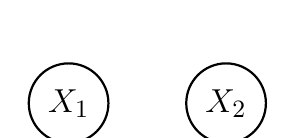
\begin{tikzpicture}[->,shorten >=1pt,auto,node distance=2cm, 
        thick,main node/.style={circle,fill=white,draw,font=\sffamily\bfseries}]

      \node[main node] (1) {$X_1$};
      \node[main node] (2) [right of=1] {$X_2$};

    \end{tikzpicture}
    \caption{Graph with two unassociated nodes.}
    \label{fig:unconnected_nodes}
\end{figure}

These nodes are not associated simply because there is no edge between them.
This can be demonstrated by considering the factorization of \( P(x_1, x_2) \)
given by the Bayesian Network Factorization:
\[
P(x_1, x_2) = P(x_1) P(x_2)
\]
This factorization immediately proves that the two nodes
\( X_1 \) and \( X_2 \) are unassociated (independent)
in this basic structure. The key assumption here is that \( P \)
is Markov with respect to the graph in Figure \ref{fig:unconnected_nodes}.

In contrast, if there is an edge between the two nodes
(as in Figure \ref{fig:connected_nodes}),
then the nodes are associated.
\begin{figure}[h]
    \centering
    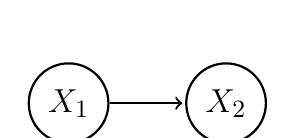
\begin{tikzpicture}[->,shorten >=1pt,auto,node distance=2cm, 
        thick,main node/.style={circle,fill=white,draw,font=\sffamily\bfseries}]

      \node[main node] (1) {$X_1$};
      \node[main node] (2) [right of=1] {$X_2$};

      \path[every node/.style={font=\sffamily\small}]
        (1) edge node {} (2);
    \end{tikzpicture}
    \caption{Graph with two nodes \(X_1\) and \(X_2\) with an arrow from \(X_1\) to \(X_2\), indicating that \(X_1\) is a cause of \(X_2\).}
    \label{fig:connected_nodes}
\end{figure}
The assumption used
here is the causal edges assumption, which indicates that
\( X_1 \) is a cause of \( X_2 \). Since \( X_1 \) is a
cause of \( X_2 \), \( X_2 \) must be able to change
in response to changes in \( X_1 \), establishing their
association. Generally, any time two nodes are adjacent
in a causal graph, they are associated.

Let's now consider more the building blocks of DAGs
as shown in Figure
\ref{fig:building}, where we have a
\textbf{chain}, a \textbf{fork} and an \textbf{immorality}.

\begin{figure}[h]
    \centering
    \includegraphics[width=\linewidth]{figures/ch3/16.building.png}
    \caption{Building blocks of DAGs: chain, fork, and immorality.}
    \vspace{-10px}
    \caption*{\scriptsize{Source: \cite{Neal_2020a}}}
    \label{fig:building}
\end{figure}

Chains and forks share the same set of dependencies.
In both structures, \(X_1\) and \(X_2\) are dependent,
and \(X_2\) and \(X_3\) are dependent for the same reason discussed
for the graph in Figure \ref{fig:connected_nodes}.
Adjacent nodes are always dependent when we make the causal edges assumption.
But does association flow from \(X_1\) to \(X_3\) through
\(X_2\) in chains and forks?

In chain graphs, \(X_1\) and \(X_3\) are usually dependent simply because
\(X_1\) causes changes in \(X_2\), which then causes changes in \(X_3\).
In a fork graph, \(X_1\) and \(X_3\) are also usually dependent
because the value that \(X_2\) takes on determines both the value that
\(X_1\) takes on and the value that \(X_3\) takes on. In other words,
\(X_1\) and \(X_3\) are associated through their shared common cause.
However, while in chains the association between \(X_1\) and \(X_3\)
is a causal one, in forks it is not.

Chains and forks also share the same set of independencies.
When we condition on \(X_2\) in both graphs,
it blocks the flow of association from \(X_1\) to \(X_3\).
This is due to the local Markov assumption; each variable can locally
depend only on its parents. Therefore, when we condition
on \(X_2\) (the parent of \(X_3\) in both graphs), \(X_3\)
becomes independent of \(X_1\) (and vice versa).

We refer to this independence as an instance of a blocked path.
These blocked paths are illustrated in Figure \ref{fig:blocked_paths}.

\begin{figure}[h]
    \centering
    \includegraphics[width=.65\linewidth]{figures/ch3/18.blocked.png}
    \caption{Blocked paths in chain and fork graphs.}
    \vspace{-10px}
    \caption*{\scriptsize{Source: \cite{Neal_2020a}}}
    \label{fig:blocked_paths}
\end{figure}

In contrast to chains and forks, in an immorality, \(X_1 \perp X_3\).
We observe that conditioning on a collider can turn a blocked path
into an unblocked path. The parents \(X_1\) and \(X_3\)
are not associated in the general population, but when we condition
on their shared child \(X_2\) taking on a specific value,
they become associated. Conditioning on the collider \(X_2\)
allows association to flow along the path
\(X_1 \rightarrow X_2 \leftarrow X_3\), despite the fact that it
does not when we do not condition on \(X_2\).
In Figure \ref{fig:immorality}, we can see the immorality with
the blocked path and the unblocked path.

\begin{figure}[h]
    \centering
    \includegraphics[width=.65\linewidth]{figures/ch3/19.immorality.png}
    \caption{Immorality with a blocked path and an unblocked path.}
    \vspace{-10px}
    \caption*{\scriptsize{Source: \cite{Neal_2020a}}}
    \label{fig:immorality}
\end{figure}

Conditioning on \textbf{descendants of a collider} also induces
association between the parents of the collider.
The intuition is that if we learn something about a collider's descendant,
we usually also learn something about the collider itself because there
is a direct causal path from the collider to its descendants.
In Figure \ref{fig:descendants}, we can see a conditioning
on a descendant of a collider.

\begin{figure}[h]
    \centering
    \includegraphics[width=.25\linewidth]{figures/ch3/20.descendant.png}
    \caption{Conditioning on a descendant of a collider.}
    \vspace{-10px}
    \caption*{\scriptsize{Source: \cite{Neal_2020a}}}
    \label{fig:descendants}
\end{figure}

Now let's formally codify the concept of a \textbf{blocked path}:
a path between nodes \( X \) and \( Y \) is \textbf{blocked} by a
(potentially empty) conditioning set \( Z \) if either of the following
is true:
\begin{enumerate}
    \item Along the path, there is a chain
    \(\cdots \rightarrow W \rightarrow \cdots\) or a fork
    \(\cdots \leftarrow W \rightarrow \cdots\),
    where \( W \) is conditioned on (\( W \in Z \)).
    \item There is a \textbf{collider} \( W \) on the path
    that is not conditioned on (\( W \notin Z \)) and none
    of its descendants are conditioned on (\( de(W) \nsubseteq Z \)).
\end{enumerate}

An \textbf{unblocked path} is simply a path that is not blocked.
The graphical intuition to have in mind is that \textbf{association} flows along
unblocked paths and does not flow along blocked paths.

Now, we are ready to introduce
\textbf{d-separation}: two (sets of) nodes \( X \) and \( Y \) are
\textbf{d-separated} by a set of nodes \( Z \) if all of the paths
between (any node in) \( X \) and (any node in) \( Y \) are blocked by \( Z \)
(\cite{pearl1988}).

Otherwise, they are \textbf{d-connected}.


\subsection{Potential Outcomes and the Fundamental Problem of Causal Inference}
\label{sec:potential_outcomes}

The central issue driving the need for causal inference is that
correlation does not imply causation. If these two concepts were equivalent,
causal inference would be easy.
This raises the critical question: how can we determine when one
event causes another and, therefore, infer causality?

To address this, we introduce the concept of \textbf{potential outcomes}.
Suppose, as shown in Figure \ref{fig:potential_outcomes},
you have a headache, and you know that taking a pill would alleviate
the headache, whereas not taking the pill would result in the
headache persisting. In this scenario, you can infer a causal effect
of the pill on the headache. However, if not taking the pill
also resulted in the headache disappearing, you would conclude
that there is no causal effect.
This is the intuition behind potential outcomes.

\begin{figure}[h]
    \centering
    \includegraphics[width=.75\textwidth]{figures/ch3/11.potential.png}
    \caption{Potential outcomes for a causal effect.}
    \vspace{-10px}
    \caption*{\scriptsize{Source: \cite{Neal_2020a}}}
    \label{fig:potential_outcomes}
\end{figure}

Let's define some notation:
\begin{itemize}
    \item \( T \): Observed treatment
    \item \( Y \): Observed outcome
    \item \( i \): Denotes a specific unit or individual
    \item \( Y_i|_{\text{do}(T=1)} \triangleq Y_i(1) \): Potential outcome under treatment
    \item \( Y_i|_{\text{do}(T=0)} \triangleq Y_i(0) \): Potential outcome under no treatment
    \item \( \text{\textbf{Causal Effect}} = Y_i(1) - Y_i(0) \)
\end{itemize}


To account for individual differences, we measure the
\textbf{Average Treatment Effect} (ATE), given by:
\begin{equation}
\mathbb{E}[Y(1)] - \mathbb{E}[Y(0)].
\end{equation}

A fundamental problem in causal inference is the challenge
of distinguishing between the observational distribution
\( P(Y|T=t) \) and the interventional distribution \( P(Y|\text{do}(T=t)) \).
These distributions are generally not equal; if they were, correlation
would indeed imply causation. The intervention \( T=t \) on a population
is denoted by the do-operator, which allows us to measure the causal
effect from the interventional distribution \( P(Y|\text{do}(T=t)) \).

However, we often cannot intervene on the entire population
and can only access the observational distribution.
The distinction between these distributions is illustrated
in Figure \ref{fig:dooperator}.
Intervening with \( \text{do}(T=0) \) (\textbf{factual}) usually
precludes access to \( \text{do}(T=1) \) (\textbf{counterfactual}).

\begin{figure}[h]
    \centering
    \includegraphics[width=\textwidth]{figures/ch3/12.dooperator.png}
    \caption{The difference between observational and interventional distributions.}
    \vspace{-10px}
    \caption*{\scriptsize{Source: \cite{Neal_2020a}}}
    \label{fig:dooperator}
\end{figure}

One approach to address this issue is
through a \textbf{Randomized Controlled Trial} (RCT). In an RCT, participants
are randomly assigned to treatment or control groups, ensuring that
\( (Y(1), Y(0)) \perp\!\!\!\perp T \), under the assumption of exchangeability.
\textbf{Exchangeability} means that the treatment groups are comparable in the
sense that if they were swapped, the new treatment group would exhibit
the same outcomes as the original treatment group, and the new control
group would exhibit the same outcomes as the original control group.
The randomization process ensures that, as we can see in Figure \ref{fig:rct},
the causal association between the treatment and the outcome is identifiable
since there is no confounding due to a missing connection between the
treatment and the cause.

\begin{figure}[h]
    \centering
    \begin{subfigure}{.5\textwidth}
      \centering
      \includegraphics[width=.8\linewidth]{figures/ch3/13.rct1.png}
    \end{subfigure}%
    \begin{subfigure}{.5\textwidth}
      \centering
      \includegraphics[width=.8\linewidth]{figures/ch3/14.rct2.png}
    \end{subfigure}
    \caption{Randomized Controlled Trial (RCT) design vs. Observational Study.}
    \vspace{-10px}
    \caption*{\scriptsize{Source: \cite{Neal_2020a}}}
    \label{fig:rct}
\end{figure}

However, it is not always feasible to randomize treatment due to several reasons:
\begin{itemize}
    \item \textbf{Ethical reasons}: For instance, it would be unethical
    to randomize people to smoke in order to measure the effect on lung cancer.
    \item \textbf{Infeasibility}: It is impractical to randomize
    countries into different economic systems
    (e.g. communist vs. capitalist) to measure the effect on GDP.
    \item \textbf{Impossibility}: Certain changes, such as altering a
    person's DNA at birth to measure the effect on breast cancer,
    are simply not possible.
\end{itemize}
We must then find a way to estimate causal effects from observational data.

\subsection{Causal Models and Identification}
\label{sec:causal_models}

\textbf{Identification} is the process of moving from a \textbf{causal estimand}
to a \textbf{statistical estimand}. As we have seen in \ref{sec:potential_outcomes},
conditioning on \( T = t \) means that we are restricting our focus to the subset
of the population who received treatment \( t \). In contrast, an \textbf{intervention}
(denoted with the \textbf{do-operator}) involves taking the entire population and
giving everyone treatment \( t \).

\textbf{Interventional distributions} such as \( P(Y \mid do(T = t)) \)
are conceptually quite different from the \textbf{observational distribution} \( P(Y) \)
since the latter do not include the do-operator.
Because of this, we can observe data from them without conducting any experiments.
This is why we call data from \( P(Y, T, X) \) \textbf{observational data}.
If we can reduce an expression \( Q \) with do in it (an interventional expression)
to one without do in it (an observational expression), then \( Q \) is said to be
\textbf{identifiable}. We will refer to an estimand as a
\textbf{causal estimand} when it contains a do-operator,
and as a \textbf{statistical estimand} when it does not contain a do-operator.

Before describing a very important assumption, we must specify what
a \textbf{causal mechanism} is,
we will refer to the causal mechanism that generates \( X_i \)
as the conditional distribution of \( X_i \) given all of
its causes: \( P(x_i \mid \text{pa}_i) \).

To achieve many causal identification results, the main assumption we will
make is that interventions are local:
intervening on a variable \( X_i \) only changes the causal mechanism for \( X_i \).
In this sense, the causal mechanisms are \textbf{modular}.

\textbf{Assumption of Modularity / Independent Mechanisms / Invariance}:\\
If we intervene on a set of nodes \( S \subseteq [n] \)\footnote{We use \( [n] \) to refer to the set \(\{1, 2, \ldots, n\}\).}, setting them to constants, then for all \( i \), we have the following:
\begin{enumerate}
    \item If \( i \notin S \), then \( P(x_i \mid \text{pa}_i) \) remains unchanged.
    \item If \( i \in S \), then \( P(x_i \mid \text{pa}_i) = 1 \) if \( x_i \)
    is the value that \( X_i \) was set to by the intervention; otherwise,
    \( P(x_i \mid \text{pa}_i) = 0 \).
\end{enumerate}

The modularity assumption allows us to encode many different interventional
distributions in a single graph. For example, it could be the case that
\( P(Y) \), \( P(Y \mid do(T = t)) \), \( P(Y \mid do(T = t')) \), and
\( P(Y \mid do(T_2 = t_2)) \) are all completely different distributions that
share almost nothing. If this were the case, each of these distributions would
need its own graph. However, by assuming modularity, we can encode them all
with the same graph that we use to encode the joint \( P(Y, T, T_2, \ldots) \),
and we can know that all of the factors (except the ones that are intervened on)
are shared across these graphs.

The \textbf{causal graph} for interventional distributions,
as shown in an example in Figure \ref{fig:intervention},
is simply the same graph used for the observational joint distribution,
but with all of the edges to the intervened node(s) removed.
This is because the probability for the intervened factor has been set to 1,
allowing us to ignore that factor.

\begin{figure}[h]
    \centering
    \includegraphics[width=\textwidth]{figures/ch3/21.intervention.png}
    \caption{Intervention as edge deletion in causal graphs.}
    \vspace{-10px}
    \caption*{\scriptsize{Source: \cite{Neal_2020a}}}
    \label{fig:intervention}
\end{figure}

Recall from subsection \ref{sec:flow}, that \textbf{causal association}
flows from \( T \) to \( Y \) along directed paths,
while \textbf{non-causal association} can flow along other
paths from \( T \) to \( Y \) unless they are blocked by either
a non-collider that is conditioned on or a collider that is not
conditioned on. These non-directed unblocked paths from
\( T \) to \( Y \) are known as \textbf{backdoor paths}
because they have an edge that goes in the ``backdoor'' of the \( T \) node.
By conditioning on certain variables, we can block these paths and
identify causal quantities like \( P(Y \mid \text{do}(T = t)) \).

Our goal is to transform the causal estimand
\( P(y \mid \textbf{do}(T = t)) \) into a statistical estimand
that relies only on the observational distribution.
We start by assuming we have a set of variables \( W \) that satisfy
the \textbf{backdoor criterion}:\\
A set of variables \( W \) satisfies the backdoor criterion relative to \( T \) and \( Y \) if the following are true:
\begin{enumerate}
    \item \( W \) blocks all backdoor paths from \( T \) to \( Y \).
    \item \( W \) does not contain any descendants of \( T \).
\end{enumerate}

When \( W \) satisfies the backdoor criterion,
it becomes a \textbf{sufficient adjustment set}.
Additionally, we must ensure \textbf{positivity},
which means that all subgroups of the data with different
covariates have some probability of receiving any value of treatment.
Formally, we define \textbf{positivity} for binary treatment as follows:\\
For all values of covariates \( x \) present in the population of
interest (i.e., \( x \) such that \( P(X = x) > 0 \)),
\[
0 < P(T = 1 \mid X = x) < 1
\]

\textbf{Backdoor Adjustment}: Given the modularity assumption,
that \( W \) satisfies the backdoor criterion, and positivity, 
we can identify the causal effect of \( T \) on \( Y \):
\begin{equation}
P(y \mid \textbf{do}(T = t)) = \sum_{w} P(y \mid T = t, W = w) P(w)
\end{equation}

This theorem connects to \textbf{d-separation}.
We can use the backdoor adjustment if \( W \)
\textbf{d-separates} \( T \) from \( Y \) in the manipulated graph.
Recall that isolating the causal association means
identifying it. We achieve this if \( T \) is d-separated from
\( Y \) in the manipulated graph or if \( Y \)
is d-separated from \( T \) in the manipulated graph,
conditional on \( W \).
In Figure \ref{fig:backdoor}, we can see how the backdoor paths
that are blocked by conditioning on \( W \) allow
us to identify the causal effect of \( T \) on \( Y \).

\begin{figure}[H]
    \centering
    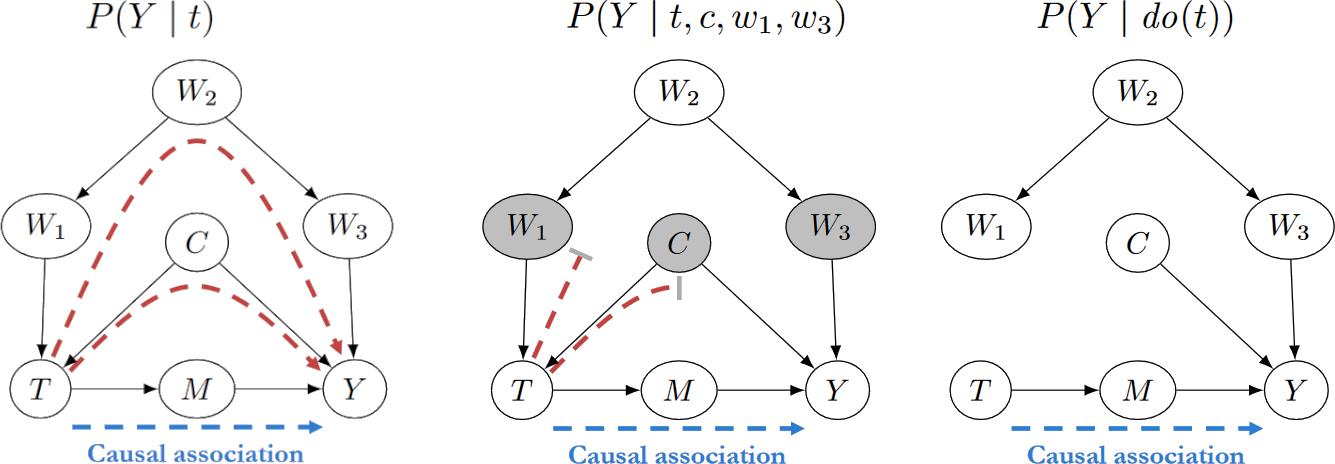
\includegraphics[width=\textwidth]{figures/ch3/22.backdoor.png}
    \caption{Backdoor paths blocked by conditioning on \( W \).}
    \vspace{-10px}
    \caption*{\scriptsize{Source: \cite{Neal_2020a}}}
    \label{fig:backdoor}
\end{figure}

\subsection{Structural Causal Models}
\label{sec:scm}

We need to be able to state that $A$ is a \textbf{cause} of $B$,
meaning that changing $A$ results in changes in $B$, but changing
$B$ does not result in changes in $A$.
This relationship is represented by the following
\textbf{structural equation}:
\begin{equation}
B := f(A) \label{eq:streq}
\end{equation}
where \( f \) is some function that maps $A$ to $B$.

However, the mapping between $A$ and $B$ in Equation \ref{eq:streq}
is \textbf{deterministic}. Ideally, we'd like to allow it to be
\textbf{probabilistic}, which allows room for some unknown
causes of $B$ that factor into this mapping.
We can then write the following:
\begin{equation}
B := f(A, U) \label{eq:strequn}
\end{equation}
where \( U \) is some unobserved random variable.
The graph for this simple structural equation is shown in Figure \ref{fig:struct_eq}.

\begin{figure}[H]
    \centering
    \includegraphics[width=.25\textwidth]{figures/ch3/23.struct_eq.png}
    \caption{Graph of \ref{eq:strequn}.
    The dashed node $U$ means that
    $U$ is unobserved.}
    \vspace{-10px}
    \caption*{\scriptsize{Source: \cite{Neal_2020a}}}
    \label{fig:struct_eq}
\end{figure}

While we have shown a single \textbf{structural equation}
in Equation \ref{eq:strequn}, there can be a large collection of
structural equations in a single model, commonly
labeled \( M \). For example, we write structural equations
for the causal model in Figure \ref{fig:scm} below:
\begin{equation}
M :
\begin{cases}
B := f_B(A, U_B) \\
C := f_C(A, B, U_C) \\
D := f_D(A, C, U_D)
\end{cases}
\label{eq:scm}
\end{equation}

\begin{figure}[H]
    \centering
    \includegraphics[width=.45\textwidth]{figures/ch3/24.scm.png}
    \caption{Graph of \ref{eq:scm}.}
    \vspace{-10px}
    \caption*{\scriptsize{Source: \cite{Neal_2020a}}}
    \label{fig:scm}
\end{figure}

The variables for which we write structural equations are known as
\textbf{endogenous variables}. These are the variables whose causal
mechanisms we are modeling.
In contrast, \textbf{exogenous variables} are variables that
do not have any parents in the causal graph.

\textbf{Structural Causal Model (SCM)}: a structural causal model
is a tuple consisting of the following sets:
\begin{enumerate}
    \item A set of endogenous variables \( V \)
    \item A set of exogenous variables \( U \)
    \item A set of functions \( f \), one to generate each
    endogenous variable as a function of other variables
\end{enumerate}

\chapter{Methodology}

\section{Problem Statement}

In this work, we address the challenge of training an agent using
an offline Deep Reinforcement Learning (DRL) algorithm with access 
to a pre-collected dataset \( \mathcal{D} \) of experiences. 
Each experience in \( \mathcal{D} \) captures an interaction with
the environment and is represented as a tuple
\[ T = (s_t, s_{t+1}, a_t, r_{t+1}) .\] Here, \( s_t \)
and \( s_{t+1} \) are the \textbf{observed states} at time-steps
\( t \) and \( t+1 \), respectively, \( a_t \) is the \textbf{action}
taken at time \( t \), and \( r_{t+1} \) is the \textbf{reward} received
after taking action \( a_t \) and transitioning to state \( s_{t+1} \).
States can be represented in various forms:
\begin{itemize}
    \item \textbf{Numerical data}: consisting of a stack of vectors of
    real numbers representing the physical state of the environment
    (e.g., position, velocity, orientation in robotics,
    suffering from anemia or not in healthcare).
    \item \textbf{Images}: consisting of a sequence of images
    observed by the agent (e.g., frames from a camera mounted on a
    robot or a patient's medical images).
    \item \textbf{Images and numerical data}: a combination of the
    above two representations (e.g., images from a robot's camera
    and its joint angles).
\end{itemize}
The number of images (or vectors) in the state representation
is denoted by \( N_{\mathcal{S}} \) such that
\[ s_t = \{ \mathcal{S}_{t-(N_{\mathcal{S}-1})}, \ldots,
\mathcal{S}_{t-1}, \mathcal{S}_t \} \text{  and  }
s_{t+1} = \{ \mathcal{S}_{t-(N_{\mathcal{S}-2})}, \ldots,
\mathcal{S}_t, \mathcal{S}_{t+1} \} \]
\[
    \text{where } \mathcal{S}_t =
    \{\text{`num': } \mathcal{X}_t, \text{ `img': } \mathcal{I}_t\} \text{ or }
    \mathcal{S}_t = \{\text{`num': } \mathcal{X}_t\}
    \text{ or } \mathcal{S}_t = \{\text{`img': } \mathcal{I}_t\}.
\]

In real-world scenarios, where comprehensive simulators are unavailable,
the dataset \( \mathcal{D} \) may lack experience due
to potential risks (e.g., collisions, patient harm) or high costs.
This deficiency can prevent the agent's training and result in policies
that are neither effective nor robust. Therefore, our goal is to \textbf{augment}
\( \mathcal{D} \) by generating additional experiences that
\textbf{align with the environment's underlying transition dynamics}.

To model these state-transition dynamics, we use a
\textbf{Structural Causal Model} (SCM)
defined as:
\[
S_{t+1} = f_s(S_t, A_t, U_{t+1})
\]
where \( S_{t+1} \), \( S_t \), and \( A_t \) are random variables representing
the states and action, while \( U_{t+1} \) represents unobserved
variables affecting the transition.
The function \( f_s \) captures the causal mechanism
determining the next state \( S_{t+1} \) from its causes
\( S_t \), \( A_t \), and \( U_{t+1} \).
Additionally, we model the reward as:
\[
R_{t+1} = f_r(S_t, S_{t+1}, A_t)
\]
If \( f_s \) and \( f_r \) are known, we can generate
\textbf{counterfactual} experiences.

Given an observed tuple \( T = (s_t, s_{t+1}, a_t, r_{t+1}) \),
we aim to create a new tuple \( T' = (s_t, s'_{t+1}, a'_t, r'_{t+1}) \)
representing what might have occurred if a different action \( a'_t \)
were taken in state \( s_t \). This involves the following steps:
\begin{enumerate}
    \item \textbf{Abduction}: Estimate \( U_{t+1} = \hat{u}_{t+1} \)
    from the observed data \( T = (s_t, s_{t+1}, a_t, r_{t+1}) \);
    \item \textbf{Action}: Perform the counterfactual action
    \( a'_t \neq a_t \);
    \item \textbf{Prediction}: Use the estimated \( \hat{u}_{t+1} \)
    and the updated SCM model to predict \( s'_{t+1} \) and \( r'_{t+1} \).
\end{enumerate}

A key question in counterfactual reasoning is whether the counterfactual
outcome is identifiable given the observed data. The following
theorem, presented in \cite{lu2020},
shows that under weak assumptions, the counterfactual outcome
is indeed identifiable.

\begin{theorem}
    Suppose the state transition $S_{t+1}$ satisfies the following SCM:
    $$S_{t+1} = f_s(S_t, A_t, U_{t+1})$$
    where $U_{t+1} \independent (S_t, A_t)$,
    and the function $f_s$ is smooth and strictly monotonic
    in $U_{t+1}$ for fixed values of $S_t$ and $A_t$.
    Suppose we have observed $\left\langle S_t = s_t, A_t = a, S_{t+1} = s_{t+1}\right\rangle $,
    then the counterfactual outcome for the counterfactual action $A_t = a'$:
    $$S_{t+1,\; A_t=a'} | S_t = s_t,\; A_t = a,\; S_{t+1} = s_{t+1}$$ is identifiable.
\end{theorem}

The strict monotonicity of $f$ in $U_{t+1}$ guarantees that the unobserved
noise term $U_{t+1}$ can be recovered from the observed
$\left\langle S_t, A_t, S_{t+1}\right\rangle $.
With the recovered $U_{t+1}$, we can then predict the counterfactual outcome
$S_{t+1,\; A_t=a'}$ by plugging in the new action $a'$ into the SCM.

This theorem holds regardless of whether the state and action spaces are
continuous or discrete, and it does not depend on the specific form of $f_s$
or the distribution of $U_{t+1}$, as long as the monotonicity condition is
satisfied.
The key insight is that the counterfactual outcome is identifiable under
weak assumptions, making counterfactual reasoning generally possible in
a wide range of models and settings.
In experiments, this strict monotonicity can be easily implemented through
a monotonic multi-layer perceptron network
while we will ensure that $U_{t+1}$ is, in fact, independent of $(S_t, A_t)$
in our environments by observing their assumed SCM graph.

By creating these counterfactual samples, we can form an augmented dataset
\( \mathcal{D}' \), which can then be used to train an offline DRL agent.

In practice, however, neither
\( f_s \) and \( f_r \), nor the function to perform
the abduction step and estimate the unobserved variable
\( U_{t+1} \) are known. In the following, we present the framework
we devised to infer the SCM model from the available data \( \mathcal{D} \)
and simultaneously learn a function to estimate
\( U_{t+1} \) (see Subsection \ref{sec:wre}). Additionally, we investigated
a method where the noise is known and counterfactual states are collected
(see Subsection \ref{sec:sctdg}).

\section{Simulation Environments}

Here we introduce the simulation environments used in our experiments,
which are essential for creating the dataset \( \mathcal{D} \) and
training the offline DRL agents.

Two categories of environments are considered: \textbf{Robotics} and
\textbf{Healthcare}.

\subsection{Robotics Environments}

\textbf{MuJoCo} (Multi-Joint dynamics with Contact)
is a physics engine developed by \cite{todorov2012mujoco}
that has become a standard tool in reinforcement learning research.
It provides a platform for simulating complex multi-joint dynamics
and it's widely used in application areas which
demand fast and accurate simulation of articulated
structures interacting with their environment.

The environments we focus on in this work are
\textbf{HalfCheetah} and \textbf{Ant},
their wrapper can be found, as initially
presented in \cite{brockman2016openaigym},
in the OpenAI Gym toolkit.
In addition to these, we also include \textbf{Acrobot},
a classic control problem also available in the OpenAI Gym
toolkit and based on the work of \cite{sutton1998}.
Its inclusion provides
a contrast to the more complex MuJoCo environments and
allows us to test our methods on a wider range of
control problems.

In these robotics environments, we can consider
various SCMs
to capture the state-transition dynamics. For example:
\begin{enumerate}
    \item $S_{t+1} = f_s(S_t, A_t, U_{t+1})$, where $U_{t+2}$
    is causally dependent on $U_{t+1}$, 
    $S_{t+1}$ is causally dependent on $S_t$ and $A_t$, and
    $A_t$ is causally dependent on $S_t$. Shown in Figure \ref{fig:scm1}.
    \item $S_{t+1} = f_s(S_t, A_t, U_{t+1})$, like on the
    the first case, but the noise terms $U_{t+i}$ are independent
    among each other. Shown in Figure \ref{fig:scm2}.
    \item $S_{t+1} = f_s(S_t, A_t, U_{t+1})$, like on the
    the first case, but $S_{t+1}$ is causally dependent on both $S_{t-1}$
    and $S_t$. Shown in Figure \ref{fig:scm3}.
    \item $S_{t+1} = f_s(S_t, A_t, U_{t+1})$, like on the
    third case, but the noise terms $U_{t+i}$ are independent
    among each other. Shown in Figure \ref{fig:scm4}.
\end{enumerate}
\begin{figure}
    \begin{subfigure}[t]{.4\textwidth}
        \centering
        \includegraphics[width=\textwidth]{figures/ch4/scm1.png}
        \caption{\nth{1} SCM}
        \label{fig:scm1}
    \end{subfigure}
    \hfill
    \begin{subfigure}[t]{.4\textwidth}
        \centering
        \includegraphics[width=\textwidth]{figures/ch4/scm2.png}
        \caption{\nth{2} SCM}
        \label{fig:scm2}
    \end{subfigure}
    \medskip
    \begin{subfigure}[t]{.4\textwidth}
        \centering
        \includegraphics[width=\textwidth]{figures/ch4/scm3.png}
        \caption{\nth{3} SCM}
        \label{fig:scm3}
    \end{subfigure}
    \hfill
    \begin{subfigure}[t]{.4\textwidth}
        \centering
        \includegraphics[width=\textwidth]{figures/ch4/scm4.png}
        \caption{\nth{4} SCM}
        \label{fig:scm4}
    \end{subfigure}
    \caption{SCMs for the robotics environments.}
\end{figure}
In all these cases, we can effectively show that
$U_{t+1} \independent (S_t, A_t)$ thanks to the rules
of \textbf{d-separation} shown in Subsection \ref{sec:causal_models}.
In Figure \ref{fig:scm-dep}, we present a visual representation
of the d-separation rules for one of the SCMs considered in this work
(these conditions hold for all the SCMs considered):
since $S_{t-1}$, $A_{t-1}$ and $U_t$ are observed and conditioned upon,
the flow of association given by their fork structure is blocked,
the only way for $U_t$ to influence $S_t$ could be
through their common child $S_{t+1}$, which is unobserved,
so the independence condition holds.

A case where the independence condition may not hold would be an
SCM of the form:
\begin{enumerate}
    \setcounter{enumi}{4}
    \item $S_{t+1} = f_s(S_t, A_t, U_{t+1})$,
    where the noise term $U_{t+1}$ depends on the concurrent action
    $A_t$. This scenario, where the action affects the noise at the same time,
    is a rather difficult condition to achieve in the simulation
    environments considered in this work. Shown in Figure \ref{fig:scm5}.
\end{enumerate}
\begin{figure}[h]
    \begin{subfigure}[t]{.41\textwidth}
        \centering
        \includegraphics[width=\textwidth]{figures/ch4/scm-dep.png}
        \caption{SCM with d-separation rules applied.}
        \label{fig:scm-dep}
    \end{subfigure}
    \hfill
    \begin{subfigure}[t]{.41\textwidth}
        \centering
        \includegraphics[width=\textwidth]{figures/ch4/scm5.png}
        \caption{\nth{5} SCM}
        \label{fig:scm5}
    \end{subfigure}
    \caption{SCMs and association rules.}
\end{figure}

We applied a
noise $\sim \text{Normal}(\mu=0.01, \sigma=1)$ on the state at each timestep
in all the robotic environments.

\subsubsection{Acrobot}

The Acrobot environment \cite{acrobotfarama} simulates a two-link
pendulum with only the second joint actuated. A screenshot of the
Acrobot environment is shown in Figure \ref{fig:acrobot}.\\
\textbf{Description}: The Acrobot system consists of two links
connected linearly to form a chain, with one end of the chain fixed
and the other end free. The joint between the two links is actuated.
The goal is to swing the free end of the chain above the fixed base
by applying torques on the actuated joint.\\
\textbf{State space}: The state space consists of 6 continuous variables:
\begin{itemize}
    \item $\cos(\alpha_t)$, $\sin(\alpha_t)$, $\cos(\beta_t)$, $\sin(\beta_t)$
    \item Angular velocity of $\alpha_t$ and $\beta_t$
\end{itemize}
The placement of the angles can be seen in Figure \ref{fig:acrobot}.
The angles are measured counterclockwise.\\
\textbf{Action space}: The action space is discrete with 3 possible actions:
\begin{enumerate}
    \item Apply a negative torque of -1 to the actuated joint
    \item Apply no torque (0) to the actuated joint
    \item Apply a positive torque of +1 to the actuated joint
\end{enumerate}
\textbf{Reward function}: The reward function is defined as:
\begin{equation}
    R = -1 \times \text{ number of timesteps (with a limit on 100)}
\end{equation}
\textbf{Termination conditions}: The episode terminates when either
the goal position is reached or the maximum number
of timesteps (500) is reached.

\begin{figure}[h]
    \centering
    \includegraphics[width=.45\textwidth]{figures/ch4/acrobotpic.png}
    \caption{Screenshot of the Acrobot environment with information about the state.}
    \vspace{-10px}
    \caption*{\scriptsize{Source: \cite{acrobotpic}}}
    \label{fig:acrobot}
\end{figure}

\subsubsection{Half Cheetah}

The Half Cheetah environment \cite{halfcheetahfarama} 
simulates a 2-dimensional robot with two paws,
a screenshot of said environment is shown
in Figure \ref{fig:halfcheetah}.\\
\textbf{Description}: The Half Cheetah is a 2-dimensional robot
composed of 9 body segments connected by 8 joints, including two paws
The objective is to apply torques to these joints to propel the
cheetah forward (to the right) as quickly as possible.
The torso and head of the cheetah remain fixed
and torque can be applied only to the other 6 joints,
which include the connections between the torso and
the front and back thighs, the thighs and shins, and the shins and feet.\\
\textbf{State space}: The state space consists of positional values
of different body parts of the Half Cheetah, followed by the velocities
of those individual parts (their derivatives), with all the positions
ordered before all the velocities.\\
\textbf{Action space}: The action space consists of $6$ continuous values
included in $[-1, 1]$,
corresponding to the torques applied to each one of the joints.\\
\textbf{Reward function}: The reward is typically
 the \textbf{forward} reward
- a reward for moving forward, minus the \textbf{ctrl} cost
- a cost for applying excessively large actions.
The reward function is defined as:
\begin{equation}
    R = \textsf{healthy\_reward} + \textsf{forward\_reward} - \textsf{ctrl\_cost}
\end{equation}
where
\begin{equation}
    \textsf{ctrl\_cost} = \textsf{ctrl\_cost\_weight} \times sum(\textsf{action}^2)
\end{equation}
and \textsf{ctrl\_cost\_weight} is a hyperparameter with a default value of $0.1$.\\
\textbf{Termination conditions}: The episode terminates if the
Half Cheetah falls over
(typically defined as when the torso's z-coordinate falls below a threshold)
or if any of the state space values is no longer finite.

\begin{figure}[h]
    \centering
    \includegraphics[width=.4\textwidth]{figures/ch4/halfcheetah.png}
    \caption{Screenshot of the Half Cheetah environment.}
    \vspace{-10px}
    \caption*{\scriptsize{Source: \cite{halfcheetahpic}}}
    \label{fig:halfcheetah}
\end{figure}

\subsubsection{Ant}

The Ant environment \cite{antfarama} simulates a four-legged robot
in a plane. A screenshot of the Ant environment
is shown in Figure \ref{fig:ant}.\\
\textbf{Description}: The Ant consists of a torso and four legs, each with
two joints, resulting in a total of $8$ actuated joints.
The goal is to coordinate the four legs to move forward (to the right)
by applying torques to the eight hinges that connect the nine body parts,
consisting of each leg's two segments and the torso.\\
\textbf{State space}: The state space consist of positional values
of different body parts of the ant, followed by the velocities
of those individual parts (their derivatives)
with all the positions ordered before all the velocities.\\
\textbf{Action space}: The action space consists of $8$ continuous values
included in $[-1, 1]$,
corresponding to the torques applied to each one of the joints.\\
\textbf{Reward function}: The reward is typically a combination
of the \textbf{healthy} reward - a fixed reward for each timestep where
the ant is alive and the \textbf{forward} reward - a reward for moving
forward, all this minus the \textbf{ctrl} cost - a cost for applying
for taking excessively large actions and, eventually, a \textbf{contact}
cost - a negative reward applied if the external contact force is too large.
The reward function is defined as:
\begin{equation}
    R = \textsf{healthy\_reward} + \textsf{forward\_reward} - \textsf{ctrl\_cost} \;[- \textsf{contact\_cost}]
\end{equation}
\textbf{Termination conditions}: The episode terminates
if the ant falls over
(typically defined as when the torso's z-coordinate falls below a threshold)
or if any of the state space values is no longer finite.

\begin{figure}[h]
    \centering
    \includegraphics[width=.4\textwidth]{figures/ch4/ant.png}
    \caption{Screenshot of the Ant environment.}
    \vspace{-10px}
    \caption*{\scriptsize{Source: \cite{antpic}}}
    \label{fig:ant}
\end{figure}

\begin{comment}

\subsubsection{Pusher}

The Pusher environment \cite{pusherfarama} simulates
a robotic arm tasked with pushing a puck to a target
location on a plane.
A screenshot of the Pusher environment is shown in Figure \ref{fig:pusher}.\\
\textbf{Description}: The Pusher consists of a
robotic arm with shoulder, elbow, forearm, and wrist joints,
and its task is to move a puck to a specified
target location on a flat surface.
The arm must apply forces to push the puck while
coordinating its own movement.\\
\textbf{State space}: The state space consists
of the angular rotation and velocities of the robotic arm's joints,
the position of the fingertips, of the puck and the position of the target.\\
\textbf{Action space}: The action space consists of $7$ continuous values,
this time given in couples $(a,b)$ - where 
$a$ and $b$ represent the torques applied at the hinge joints,
included in $[-2, 2]$.\\
\textbf{Reward function}: The reward consists of three components:
\textbf{near} reward - which measures the distance between the
pusher's fingertip and the object as a negative vector norm
($-norm(\textsf{fingertip} - \textsf{target})$),
\textbf{dist} reward - which measures the distance between
the object and the target goal calculated as a negative norm
($- norm(\textsf{object} - \textsf{target})$)
and \textbf{control} reward - which penalizes large actions
and is calculated as the negative squared Euclidean norm of the action
($- sum(\textsf{action}^2)$). The total reward is:
\begin{equation}
    R = \textsf{reward\_dist} + 0.1 \times \textsf{reward\_control} + 0.5 \times \textsf{reward\_near}
\end{equation}
\textbf{Termination conditions}: The episode terminates when the puck
reaches the target location, when 100 timesteps are reached
or when any of the state space values is no longer finite.

\begin{figure}[h]
    \centering
    \includegraphics[width=.4\textwidth]{figures/ch4/pusher.png}
    \caption{Screenshot of the Pusher environment.}
    \vspace{-10px}
    \caption*{\scriptsize{Source: \cite{pusherpic}}}
    \label{fig:pusher}
\end{figure}

\end{comment}

\subsection{Healthcare Environments}

The only healthcare environment we focus on in this work is
the \textbf{Diabetes} environment.

\subsubsection{Diabetes}

In our study, we employ a simulated dataset that models
the progression of type II diabetes and the effects of antiglycaemic drugs,
as seen in \cite{sim2012}.
This simulation represents a simplified version of a longitudinal
medical study with time-varying confounders.

The key features of the simulated dataset:
\begin{enumerate}
    \item Variables:
    \begin{itemize}
        \item $U_0$: Binary indicator of subject's health status
        prior to randomization (unmeasured)
        \item $A_0,\; A_1$: Binary indicators for antiglycaemic
        drug prescription at visits 0 and 1 (actions)
        \item $L_1$: Binary indicator for anaemia at visit 1 (state)
        \item $Y$: $\log HbA_{1c}$ measured at visit 2 (outcome) (final state)
    \end{itemize}

    \item Data generation process:
    \begin{itemize}
        \item $U_0 \sim \text{Bernoulli}(0.4)$
        \item $A_0 \sim \text{Bernoulli}(0.5)$ (randomized initial treatment)
        \item $L_1 | U_0, A_0 \sim \text{Bernoulli}(P(L_1 = 1) = 0.25 + 0.3A_0 - 0.2U_0 - 0.05A_0U_0)$
        \item $A_1 | A_0, L_1 \sim \text{Bernoulli}(P(A_1 = 1) = 0.4 + 0.5A_0 - 0.3L_1 - 0.4A_0L_1)$
        \item $Y | U_0, A_0, A_1 \sim \text{Normal}(\mu = 2.5 - 0.5A_0 - 0.75A_1 + 0.2A_0A_1 - U_0, \sigma = 0.2)$
    \end{itemize}
\end{enumerate}

We want to estimate the counterfactual mean of \( Y \) under
different treatment strategies \( (a_0, a_1) \).

The counterfactual means are calculated by averaging over the
distribution of \( U_0 \):
\begin{equation}
\mathbb{E}[Y(a_0, a_1)] = 2.5 - 0.4 - 0.5a_0 - 0.75a_1 + 0.2a_0a_1.
\end{equation}
Alternatively, given \( U_{0,i} \), the potential outcomes
\( Y_i(a_0, a_1) \) can be considered as being independently
generated for each \((a_0, a_1)\) and for each \(i\) from
a normal distribution with a mean of
\( 2.5 - 0.5a_0 - 0.75a_1 + 0.2a_0a_1 + U_{0,i} \)
and a standard deviation of $0.2$.

In Figure \ref{fig:diabetes1} the SCM for the diabetes dataset
is presented.
\begin{figure}[h]
    \centering
    \includegraphics[width=.21\textwidth]{figures/ch4/diabetes1.png}
    \caption{Structural Causal Model for the diabetes dataset.}
    \vspace{-10px}
    \caption*{\scriptsize{Source: \cite{sim2012}}}
    \label{fig:diabetes1}
\end{figure}
We can notice that the data generation model for $A_0$ and $A_1$
do not incorporate $U_0$, thus $A_0 \independent U_0$ and
$A_1 \independent U_0 | L_1$. Because of this
the variation in $Y(a_0,a_1)$ is independent
of all the other random variables in the model,
making $A_0 \independent Y(a_0,a_1)$ and
$A_1 \independent Y(a_0,a_1) | A_0, L_1$.
Given this, the ``no unmeasured confounding'' assumption
hold in this case.

The return value given to the RL agent in this environment
is the reciprocal value of \( Y \) at the end of the simulation.

This dataset captures key aspects of diabetes treatment, including:
\begin{itemize}
    \item The effect of initial health status on anaemia risk
    and $HbA_{1c}$ levels
    \item The potential side effect of antiglycaemic drugs causing anaemia
    \item The influence of anaemia on subsequent treatment decisions
    \item The causal effect of treatment on $HbA_{1c}$ levels
\end{itemize}
In Figure \ref{fig:diabetes2}, we present a tree
depicting the expected values of the variables out of
a total of $2000$ subjects.

\begin{figure}[h]
    \centering
    \includegraphics[width=.65\textwidth]{figures/ch4/diabetes2.png}
    \caption{Tree diagram of the expected numbers
    along each branch for the distribution from which the diabetes
    dataset was generated.}
    \vspace{-10px}
    \caption*{\scriptsize{Source: \cite{sim2012}}}
    \label{fig:diabetes2}
\end{figure}

\section{Frameworks for Counterfactual Data Generation}

In this section, we introduce two different approaches designed to
address the challenges of training agents using Offline
Deep Reinforcement Learning (DRL) with a pre-collected dataset \( \mathcal{D} \).
Both approaches aim to generate additional high-fidelity experiences
that align with the environment's underlying transition dynamics
but differ in their methodologies and assumptions.

In the following subsections, we'll explore the specifics
of each approach, outlining their methodologies, advantages, and
implementation details. This exploration aims to
provide a comprehensive understanding of how these
frameworks can be employed to augment the dataset \( \mathcal{D} \) and improve
the training of offline DRL agents.

\subsection{Wasserstein Reward-enhanced CounTerfactual\\ Data Generation}
\label{sec:wre}

The first approach, called \textbf{Wasserstein Reward-enhanced CounTerfactual Data Generation}
(WRe-CTDG),
focuses on inferring the Structural Causal Model
(SCM) from the available data \( \mathcal{D} \) and simultaneously learning
a function to estimate the unobserved variables $U_{t+1}$.

This approach is valuable when the underlying dynamics of the
environment are complex and not fully known, allowing us to
infer and utilize causal relationships for better training.

The proposed strategy for estimating the Structural Causal Model (SCM)
integrates two key components: an optional Convolutional AutoEncoder (CAE)
for dimensionality reduction and a Deep Generative Model for
implementing the causal mechanisms.

The CAE is designed to compress high-dimensional visual inputs,
making the data more manageable while retaining essential information.
The Deep Generative Model is used to learn the causal mechanism \( f_s \),
the abduction function needed to estimate \( U_{t+1} \),
and the reward model \( f_r \).
Figure \ref{fig:wre} provides a visual illustration of the entire solution.

\begin{figure}[ht]
    \centering
    \includegraphics[width=.95\textwidth]{figures/ch4/1.wre.pdf}
    \caption{WRe-CTDG framework in a situation where the states are
    images only and the CAE is employed.}
    \label{fig:wre}
\end{figure}

\subsubsection{Dimensionality Reduction via Convolutional AutoEncoders}

Unlike state-of-the-art approaches, our work generates experience samples
where states can also be represented by images. To handle the challenges posed
by high-dimensional visual data, we present the possibility of using a CAE,
which is a Variational AutoEncoder (VAE, see Section \ref{sec:vae})
made by two Convolutional Neural Networks (CNN, see Section \ref{sec:cnn}).
to compute low-dimensional encodings that preserve the meaningful
information from the input images.
It consists of an encoder \( \phi = E_s(\mathcal{I}) \)
that extracts a low-dimensional encoding \( \phi \)
from the image \( \mathcal{I} \), and a decoder
\( D_s(\phi) = \mathcal{I}_{\text{rec}} \)
that reconstructs the original image \( \mathcal{I} \).

The CAE is trained by minimizing the reconstruction error over
the images \( \mathcal{I} \) in the collected dataset \( \mathcal{D} \):

\begin{equation}
\mathcal{L}_{E_s, D_s} = \mathbb{E}_{\mathcal{I} \sim P_{\text{data}}}
\left[ \| \mathcal{I} - \mathcal{I}_{\text{rec}} \|^2 \right]
\end{equation}

Minimizing this reconstruction error ensures that the encoder \( E_s \)
computes robust and informative image encodings and the decoder \( D_s \)
can accurately reconstruct images from these encodings.

The encoder is used to encode the images representing the environment
states into their corresponding low-dimensional encodings.
We refer to the encoded states at time \( t \) and \( t+1 \) as
\( s_{t,\phi} = E_s(s_t) \) and \( s_{t+1,\phi} = E_s(s_{t+1}) \).
The decoder is used to reconstruct images from the low-dimensional
encodings generated by the generator network. The weights of both
\( E_s \) and \( D_s \) are frozen and not updated during the next
phase of learning the SCM model.

In the next section we are not going to explicitly use
\( s_{t,\phi} \) and \( s_{t+1,\phi} \) since utilizing the
CAE is optional and depends on the nature of the state representation.
So, by default, we will refer to the states as \( s_t \) and \( s_{t+1} \).

\subsubsection{Counterfactual Data Generation}

To learn the SCM from the collected dataset \( \mathcal{D} \),
we propose a novel strategy called
Wasserstein Reward-enhanced Counterfactual Data Generation (WRe-CTDG).
This solution builds upon the BiCoGAN framework presented in \cite{lu2020}
with significant enhancements
aimed at improving the effectiveness of the estimated SCM in generating
counterfactual samples in vision-based DRL problems. Key enhancements
include adapting the Wasserstein Generative Adversarial Network (WGAN)
framework (see Section \ref{sec:wgan})
for improved training stability and introducing an additional
loss term to learn the reward model and predict reward values for counterfactual
actions.

The WRe-CTDG framework consists of three main components:

\begin{itemize}
    \item \textbf{Generator \( G_s \)}:
    Implements the causal mechanism \( f_s \).
    It maps the inputs \( (U_{t+1}, X_t) \)
    to the next-state encoding \( \hat{\phi}_{t+1} \),
    where \( X_t = (S_t, A_t) \).
    The distribution learned by \( G_s \) is
    \( P(\hat{\Phi}_{t+1} | U_{t+1}, X_t) \).
    \item \textbf{Encoder \( E_u \)}: Implements the abduction function.
    It maps the inputs \( (\Phi_{t+1}, X_t) \) to the
    estimated unobserved factor \( \hat{u}_{t+1} \).
    The distribution learned by \( E_u \) is
    \( P(\hat{U}_{t+1} | \Phi_{t+1}, X_t) \).
    Additionally, \( E_u \) estimates the reward model \( f_r \)
    to predict the reward associated with a \( (\Phi_{t+1}, X_t) \)
    tuple, denoted as \( \hat{r}_{t+1} \).
    \item \textbf{Critic \( C \)}: Integrates the WGAN paradigm
    into the framework. It replaces the discriminator in
    traditional GANs and computes a score quantifying
    the likelihood of the input tuples being drawn
    from either the joint distribution
    \( P(\hat{\Phi}_{t+1}, U_{t+1}, X_t) \) (generated samples) or
    \( P(\Phi_{t+1}, \hat{U}_{t+1}, X_t) \) (real samples).
    
    The metric is approximated by the Wasserstein distance \( W \)
    as follows:
    \begin{equation}
        \begin{aligned}
            W &=& \mathbb{E}_{T \sim P_{\mathcal{D}}} \left[ C(\hat{\Phi}_{t+1}, U_{t+1}, X_t) \right] \\ 
            & &- \mathbb{E}_{T \sim P_{\mathcal{D}}} \left[ C(\Phi_{t+1}, \hat{U}_{t+1}, X_t) \right]
        \end{aligned}
    \end{equation}
    where $C(\cdot)$ is a score computed by the critic.
\end{itemize}

The goal of training the encoder-generator pair is to minimize \( W \),
thereby improving the ability of both the encoder and generator
to produce samples that are indistinguishable from those generated
by their counterparts. Additionally, the function \( E_u \) must
accurately predict the rewards for each transition.
Thus, the objective function for the pair \( (G_s, E_u) \) is defined as:

\begin{equation}
L_{G_s, E_u} = -W + \lambda_R \; \mathbb{E}_{R_{t+1} \sim P_{\mathcal{D}}}
\left[ \| \hat{R}_{t+1} - R_{t+1} \|^2 \right]
\end{equation}

where \( \lambda_R \) regulates the influence of the reward
prediction term. On the other hand, the critic is trained
using the Wasserstein Loss with Gradient Penalty,
which addresses the problem of vanishing gradients and
the limited expressive power of traditional WGANs \cite{gulrajani2017}.
The objective function for \( C \) is defined as:

\begin{equation}
L_C = W + \lambda_G \mathbb{E}_{T \sim P_{\mathcal{D}}}
\left[ (\| \nabla_{\tilde{\Phi}_T, \tilde{U}_T} C(\tilde{\Phi}_T,
\tilde{U}_T, X_t) \| - 1)^2 \right]
\end{equation}

where \( \lambda_G \) determines the strength of the Gradient Penalty
and the interpolation variables \( \tilde{\Phi}_T \) and \( \tilde{U}_T \)
are given by:

\[
    \begin{aligned}
        \tilde{\Phi}_T \;\; &=& \alpha \, \Phi_{t+1} + (1 - \alpha) \, \hat{\Phi}_{t+1} \\ 
        \tilde{U}_T \;\; &=& \alpha \, U_{t+1} + (1 - \alpha) \, \hat{U}_T
    \end{aligned}
\]

for \( \alpha \in [0, 1] \), sampled uniformly at random,
indicating a blend between real and generated samples.
By maximizing \( W \), the critic aims to increase the difference
in evaluations between samples generated from the generator distribution
\( P(\hat{\Phi}_{t+1} | U_{t+1}, X_t) \) and those from the encoder
distribution \( P(\hat{U}_{t+1} | \Phi_{t+1}, X_t) \).

When the data is purely numerical or when the
CAE is employed, both the Generator $G_s$ and the
Encoder $E_u$ consist exclusively of fully connected
layers. This architecture is sufficient to handle
the numerical input and effectively capture the dependencies
in the data. However, when the state representation
includes images and the CAE is not employed,
convolutional layers are incorporated
into both the Generator and the Encoder:
\begin{itemize}
    \item In the Encoder, the convolutional blocks perform a
    downsampling on the images, effectively reducing their
    spatial dimensions while capturing essential features.
    These downsampled feature maps are then flattened
    and combined with the other numerical data,
    ensuring a comprehensive representation of the input.

    \item In the Generator, after extracting the numerical data,
    convolutional blocks are used to upsample the output of
    the fully connected network. This upsampling process
    reconstructs the spatial dimensions,
    enabling the model to generate the image $\mathcal{I}_{t+1}$.
\end{itemize}

\subsubsection{Experience Generation through Counterfactual Augmentation}

After understanding the causal mechanism \( f_s \),
the abduction function, and the reward model \( f_r \),
we can utilize WRe-CTDG and (optionally) the CAE
for counterfactual
data augmentation. The original dataset \( \mathcal{D} \)
is expanded by a factor of \( \beta \)
according to the method described in Algorithm \ref{alg1}.
Specifically, if the CAE is used, for each sampled tuple
\( T = (s_t, s_{t+1}, a_t, r_{t+1}) \in D \),
the image encodings in $s_t$, so
\( s_t[\text{`img'}] = \{\mathcal{I}_{t-(N_{\mathcal{S}}-1)}, \ldots, \mathcal{I}_{t-1}, \mathcal{I}_t\} \),
and \( \mathcal{I}_{t+1} \in s_{t+1} \) are first computed using
the encoder \( E_s \). Next, \( E_u \) and \( G_s \)
are used to create a counterfactual
sample through three steps:
\begin{enumerate}
    \item Perform abduction with \( E_u \) to estimate
    the unknown factor \( \hat{u}_{t+1} \);
    \item Use \( G_s \) to generate the counterfactual
    states \( \hat{s}'_{t+1} \) given
    \( \hat{u}_{t+1}, s_t \), and the counterfactual
    action \( a'_t \);
    \item Use \( E_u \) again to produce the reward
    \( \hat{r}'_{t+1} \).
\end{enumerate}

Finally, if the CAE is used,
the image \( \hat{\mathcal{I}}'_{t+1} \) is generated using
the decoder \( D_s \). Once the augmented dataset
\( \mathcal{D}' \)
is ready, it can be used to train any off-policy DRL
algorithm, such as D3QN or TD3.

\begin{algorithm}[hb]
    \small
    \caption{WRe-CTDG + CAE Counterfactual Augmentation} \label{alg1}
    
    \vspace{1pt}
    \KwIn{dataset $\mathcal{D}$, augmentation factor $\beta > 1$, \\
    ($E_s$, $D_s$) CAE, ($G_s$, $E_u$) WRe-CTDG}
    \KwOut{augmented dataset $\mathcal{D}'$}
    
    
    \BlankLine
    $\mathcal{D'} \gets copy(\mathcal{D})$ \\
    $M \gets$ size of $\mathcal{D}$ \\
    $M' = M \gets$ size of $\mathcal{D'}$ \\
    \While{$M' < \beta M$}{
        Sample batch $B$ $\in \mathcal{D}$ \\
            $B' \gets \emptyset$ 
            
            \ForEach{$ T = (s_t, s_{t+1}, a_t, r_{t+1}) \in B$}{
                \If{CAE is used}{
                    $s_{t} \gets \text{encode images in $s_{t}$:} \, E_s(s_t)$ \\
                    $s_{t+1} \gets \text{encode last image in $s_{t+1}$:} \, E_s(s_{t+1})$
                }
                \textit{Abduction}: $\hat{u}_{t+1} \gets E_u(s_{t+1}, s_{t}, a_t)$ \\
                \textit{Action}: $a'_t \gets \text{choose random action} \neq a_t $ \\
                \textit{Prediction}: $\hat{s}'_{t+1} \gets G_s(\hat{u}_{t+1}, s_{t}, a'_t)$ \\
                $\hat{r}'_{t+1} \gets E_u(\hat{s}'_{t+1}, s_{t}, a'_t)$ \\
                \If{CAE is used}{
                    $\hat{s}'_{t+1} \gets \text{decode last generated image in }\hat{s}'_{t+1} \text{ : } \, D_s(\hat{s}'_{t+1})$ \\ 
                }
                Insert $T' = (s_t, \hat{s}'_{t+1}, a'_t, \hat{r}'_{t+1})$ in $B'$ \\
            }
    
        Insert $B'$ in $\mathcal{D}'$ \\
        $M' \gets$ size of $\mathcal{D}'$
    }
    
    \BlankLine
    \Return $\mathcal{D}'$
    \vspace{2pt}
\end{algorithm}

\subsection{Supervised CounTerfactual Data Generation}
\label{sec:sctdg}

The second approach, which is called \textbf{Supervised CounTerfactual Data Generation} (S-CTDG),
assumes that the noise in the system is known
in the training phase and focuses on directly collecting
counterfactual states.

This approach is particularly useful when there is access to detailed
knowledge about the noise in a subset of the available data,
enabling a more precise simulation of the environment.
The key condition is that the rest of the dataset with unobserved
variables should exhibit similar noise behavior, allowing the model
to generalize effectively.

\begin{figure}[ht]
    \centering
    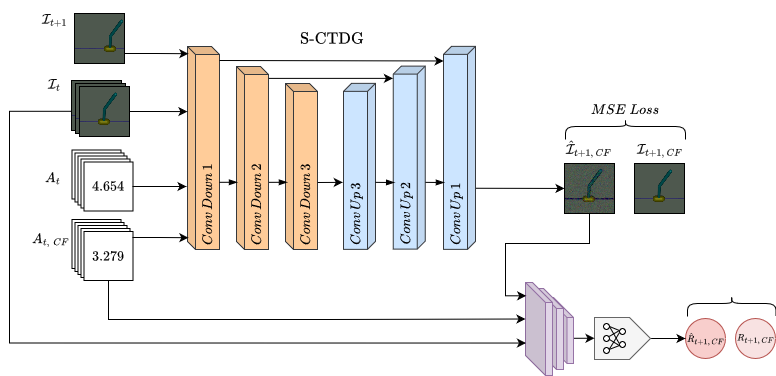
\includegraphics[width=\textwidth]{figures/ch4/2.sctdg.png}
    \caption{S-CTDG framework in a situation where the states are
    images only.}
    \label{fig:sctdg}
\end{figure}

\subsubsection{Counterfactual Data Generation}

The current architecture of our network is designed to process unimodal data,
specifically either image-based or numerical inputs.
While the framework possesses the potential for extension
to multimodal environments, the present implementation focuses
on these two distinct data types.

For \textbf{numerical data} processing, the network employs a fully connected MLP.
This network accepts as input the concatenation of the current state
$\mathcal{X}_{t}$, the subsequent state $\mathcal{X}_{t+1}$,
the action taken $A_t$, and the counterfactual action $A_{t,\, CF} \neq A_t$.
The network then produces as output the estimated counterfactual next state
$\hat{\mathcal{X}}_{t+1,\; CF}$ and the corresponding counterfactual
reward $\hat{R}_{t+1,\; CF}$.

For \textbf{image-based} inputs, we implement a CNN
architecture with symmetric downsampling and upsampling paths,
interconnected via skip connections. This structure is reminiscent
of \textbf{U-Net} introduced in \cite{ronneberger2015u},
facilitating the preservation of
spatial information.
The network's input comprises the current state image $\mathcal{I}_{t}$,
the subsequent state image $\mathcal{I}_{t+1}$,
and image representations of both the actual action $A_t$
and the counterfactual action $A_{t,\, CF} \neq A_t$. The action-to-image
conversion process is contingent on the nature of the action space:
\begin{itemize}
    \item For \textbf{discrete}, one-hot encoded action spaces (e.g. Acrobot),
    each action is represented as a single-channel image where all
    pixels hold the same value derived from the encoding vector.
    \item For \textbf{continuous} action spaces (e.g. Half Cheetah), 
    each action vector is transformed into a multi-channel image,
    where the $i$-th channel is a uniform grid populated with the
    $i$-th component of the action vector.
\end{itemize}
The network produces the counterfactual next state image
$\hat{\mathcal{I}}_{t+1,\; CF}$, which
is then processed, along with the current state image
$\mathcal{I}_{t}$ and the image representation of the counterfactual
action $\mathcal{A}_{t,\, CF}$, by a subsequent, more compact CNN.
This secondary network estimates the counterfactual reward $\hat{R}_{t+1,\; CF}$.

The loss function used to train the neural network is composed of
two terms: the Mean Squared Error (MSE) between the predicted
counterfactual state and the real counterfactual state and the
MSE between the predicted counterfactual reward and the real
counterfactual reward:
\begin{equation}
    \mathcal{L} = \mathbb{E} \left[ \left( \hat{\mathcal{S}}_{t+1,\, CF} - \mathcal{S}_{t+1,\, CF} \right)^2 \right] +
    \mathbb{E} \left[ \left( \hat{R}_{t+1,\, CF} - R_{t+1,\, CF} \right)^2 \right]
\end{equation}
where $\mathcal{S}$ represents the state as a numerical vector,
an image vector or a multimodal vector.

The S-CTDG model takes as input the current state $s_t$,
the next state $s_{t+1}$, the original action $a_t$,
and the counterfactual action $a_t'$. It then produces a counterfactual
next state $\hat{s}_{t+1}'$ and a counterfactual reward $\hat{r}_{t+1}'$.
This process effectively allows the algorithm to ask ``what if?''
questions about the environment, simulating alternative scenarios
that could have occurred if different actions
had been taken. 

\subsubsection{Experience Generation through Counterfactual Augmentation}

After understanding the end-to-end causal mechanism of the S-CTDG model,
we can utilize it for counterfactual data augmentation.
The original dataset $\mathcal{D}$ is expanded by a factor of $\beta$
according to the method described in Algorithm \ref{alg2}.
For each sampled tuple
$T = (s_t, s_{t+1}, a_t, r_t) \in \mathcal{D}$,
the process is simplified compared to the WRe-CTDG method.
Instead of separate encoding and generation steps,
the S-CTDG model $G_{sup}$ directly generates the counterfactual
state $\hat{s}_{t+1}'$ and reward $\hat{r}_{t+1}'$
given the current state $s_t$, next state $s_{t+1}$,
current action $a_t$, and a randomly chosen counterfactual action $a'_t$.
The abduction step here is implicit in the generation process.
This end-to-end approach eliminates the need for explicit
separate estimation of unknown factors.
Once the augmented dataset $\mathcal{D}'$ is ready, it can be used to
train any off-policy DRL algorithm, such as D3QN or TD3.

\begin{algorithm}[hb]
    \small
    \caption{S-CTDG Counterfactual Augmentation} \label{alg2}
    
    \vspace{1pt}
    \KwIn{dataset $\mathcal{D}$, augmentation factor $\beta > 1$, $G_{sup}$
    S-CTDG}
    \KwOut{augmented dataset $\mathcal{D}'$}
    
    
    \BlankLine
    $\mathcal{D'} \gets copy(\mathcal{D})$ \\
    $M \gets$ size of $\mathcal{D}$ \\
    $M' = M \gets$ size of $\mathcal{D'}$ \\
    \While{$M' < \beta M$}{
        Sample batch $B$ $\in \mathcal{D}$ \\
            $B' \gets \emptyset$ 
            
            \ForEach{$ T = (s_t, s_{t+1}, a_t, r_t) \in B$}{
                \textit{Action}: $a'_t \gets \text{choose random action} \neq a_t $ \\
                \textit{Prediction}: $(\hat{s}'_{t+1}, \hat{r}'_{t+1}) \gets G_{sup} (s_t, s_{t+1}, a_t, a'_{t})$ \\
                Insert $T' = (s_t, \hat{s}'_{t+1}, a'_t, \hat{r}_{t+1}')$ in $B'$ \\
            }
    
        Insert $B'$ in $\mathcal{D}'$ \\
        $M' \gets$ size of $\mathcal{D}'$
    }
    
    \BlankLine
    \Return $\mathcal{D}'$
    \vspace{2pt}
\end{algorithm}

\chapter{Experiments}

\section{Hardware Specifications}

All experiments were conducted on a high-performance
PC with the following specifications: 

\begin{itemize}
    \item CPU: Intel Core i7-9800X CPU @ 3.80GHz,
    3792 Mhz, 8 core, 16 threads
    \item GPU: 2 NVIDIA RTX 2080 Ti GPU with 12GB
    VRAM each
    \item RAM: 64 GB DDR4
    \item Storage: 1 TB Seagate BarraCuda HDD
\end{itemize}

\section{Software Environment}

The experiments were implemented using the following software stack:

\begin{itemize}
    \item Operating System: Windows 11 Pro
    \item Python: 3.10.14
    \item PyTorch: 2.3.0
    \item CUDA: 12.0
    \item TorchRL: 0.4.0
    \item MuJoCo: 3.14
\end{itemize}

\section{Network Architectures Details}

\subsection{WRe-CTDG Network Structure}

The WRe-CTDG framework consists of three main components:
Encoder $E_u$, Generator $G_s$, and Critic $C$.
Here are the details of each network:\\
\textbf{Encoder $\mathbf{E_u}$:}
\begin{itemize}
    \item Input layer: 2 $\times$ numerical state dimensions
    + 2 $\times$ latent state dimensions + action dimension
    \item Hidden layers: 4 fully connected layers with 256, 512, 512, and 256 units respectively
    \item Output layer: noise dimension + 1 (for reward prediction)
    \item Activation function: ReLU for hidden layers,
    Tanh/Sigmoid/Identity for reward output, Linear for noise output
\end{itemize}
\textbf{Generator $\mathbf{G_s}$:}
\begin{itemize}
    \item Input layer: numerical state dimension
    + latent state dimension + action dimension +
    noise dimension
    \item Hidden layers: 4 fully connected layers
    with 256, 512, 256, and 128 units respectively
    \item Output layer: numerical state dimension
    + latent state dimension
    \item Activation function: ReLU for hidden layers,
    Linear for output layer
\end{itemize}
\textbf{Critic $\mathbf{C}$:}
\begin{itemize}
    \item Input layer: 2 $\times$ numerical state dimensions
    + 2 $\times$ latent state dimensions + action dimension
    + noise dimension
    \item Hidden layers: 4 fully connected layers with 256,
    512, 256, and 128 units respectively
    \item Output layer: 1
    \item Activation function: ReLU
    for hidden layers, Linear for output layer
\end{itemize}
For environments with image inputs, we additionally used a
Convolutional AutoEncoder architecture to
encode and decode the state representations:\\
\textbf{Convolutional Encoder:}
\begin{itemize}
    \item 5 downsampling blocks
    \item Each block contains 2-3 convolutional layers
    with BatchNorm and ReLU activation
    \item Number of filters increases progressively:
    $$ in\_channels \rightarrow base \rightarrow 2
    \times base \rightarrow 4\times base \rightarrow
    8\times base \rightarrow 16\times base $$
    with $base = 8$.
    \item MaxPool2D with kernel size $2\times 2$ and stride
    2 for downsampling between blocks
    \item Final $1\times 1$ convolutional layer to
    reduce channel dimension to $bn = 1$ (bottleneck)
\end{itemize}
\textbf{Convolutional Decoder:}
\begin{itemize}
    \item Initial $1\times 1$ convolutional layer 
    to expand channel dimension from $bn$ to $16 \times base$
    \item 5 upsampling blocks
    \item Each block contains 2-3 convolutional
    layers with BatchNorm and ReLU activation
    \item Number of filters decreases progressively:
    $$ 16\times base \rightarrow 8
    \times base \rightarrow 4\times base \rightarrow
    2\times base \rightarrow base \rightarrow in\_channels$$
    with $base = 8$.
    \item Upsampling using transposed convolution
     with kernel size $2\times 2$ and stride 2
    \item Final layer uses Tanh activation
\end{itemize}
The encoder and decoder are symmetric, with the number of filters changing at each level.

\subsection{S-CTDG Network Structure}

The S-CTDG framework for \textbf{images} employs a network architecture
consisting of two components: a convolutional U-Net for counterfactual
image generation
and a separate convolutional network with a fully connected head for
reward prediction.\\
\textbf{U-Net}:
\begin{itemize}
    \item 5 downsampling blocks and 5 upsampling blocks
    \item Each block contains 2-3 convolutional layers
    with BatchNorm and ReLU activation
    \item Number of filters increases
    progressively in downsampling:
    $$ in\_channels \times (1 + stack\_length) + 2 \times (action\_channels)
    \rightarrow $$$$\rightarrow base \rightarrow 2
    \times base \rightarrow 4\times base \rightarrow
    8\times base \rightarrow 16\times base $$
    where the first term is the stack of current and previous images
    concatenated along the channel dimension with the next state image
    and the action and counterfactual action images.
    The number of filters then decreases in upsampling:
    $$ 16\times base \times 2 \rightarrow 8 \times base \times 2 \rightarrow
    4\times base \times 2\rightarrow$$ $$ \rightarrow 2\times base \times 2
    \rightarrow base \times 2 \rightarrow in\_channels$$
    with $base = 64$, in upsampling the filters are doubled
    since we concatenate the corresponding downsampling block.
    \item Convolution with kernel size $3\times 3$, stride 1,
    and padding 1
    \item MaxPool2D with kernel size $2\times 2$ and stride
    2 for downsampling between blocks
    \item Final layer uses a Softsign activation function
\end{itemize}
\textbf{Reward Prediction Network}:
\begin{itemize}
    \item 5 downsampling blocks
    \item Each block contains 2-3 convolutional layers
    with BatchNorm and ReLU activation
    \item Number of filters increases
    progressively in downsampling:
    $$ in\_channels \times (1 + stack\_length) + action\_channels
    \rightarrow base \rightarrow$$$$\rightarrow 2
    \times base \rightarrow 4\times base \rightarrow
    8\times base \rightarrow 16\times base $$
    where the first term is the stack of current and previous images
    concatenated along the channel dimension with the
    estimated counterfactual next state image
    and the counterfactual action image.
    As before, $base = 64$.
    \item Convolution with kernel size $3\times 3$, stride 1,
    and padding 1
    \item MaxPool2D with kernel size $2\times 2$ and stride
    2 for downsampling between blocks
    \item Final layer uses an Identity activation function
\end{itemize}

The S-CTDG framework for \textbf{numerical} data
employs a network architecture consisting of a single
fully connected network branched into two heads:
one for counterfactual data generation
and one for reward prediction.
The network architecture is as follows:
\begin{itemize}
    \item Input layer: 2 $\times$ numerical state dimensions
    $ + $ $2 \times $ action dimension
    \item Hidden layers: 7 fully connected layers with
    512, 512, 512 and 256 units respectively
    \item Output layer for counterfactual data generation:
    numerical state dimension, Linear activation function
    \item Output layer for reward prediction: 1,
    Identity activation function
\end{itemize}

\subsection{Reinforcement Learning Algorithms (D3QN and TD3)}

For the reinforcement learning algorithms, we used the following architectures:\\
For discrete action spaces we used \textbf{D3QN:}
\begin{itemize}
    \item Input layer: state dimension
    \item Hidden layers: 4 fully connected layers with 32, 64, 128 and 128
    units respectively
    \item Output layer: action dimension
\end{itemize}
It is a \textbf{Dueling CNN DQNetwork} as presented in \cite{d3qn}.\\
Then, for continuous action spaces we used \textbf{TD3:}\\
Actor:
\begin{itemize}
    \item Input layer: state dimension
    \item Hidden layers: 3 fully connected layers with 32, 64, 128 and 128
    units respectively
    \item Output layer: action dimension
    \item Activation function: ReLU for hidden layers, Tanh for output layer
\end{itemize}
Critic:
\begin{itemize}
    \item Input layer: state dimension + action dimension
    \item Hidden layers: 3 fully connected layers with 32, 64, 128 and 128
    units respectively
    \item Output layer: 1
    \item Activation function: ReLU for hidden layers, Linear for output layer
\end{itemize}
The actor and critic networks are modelled after
the architectures presented in \cite{lillicrap2019}. 

\section{Training Process Details}

\subsection{Dataset Generation}

For each environment, we generated a dataset of transitions using a random policy.
This dataset served as the basis for our counterfactual
data generation and reinforcement learning experiments.

The number of transitions in the dataset was different for each environment:
\begin{itemize}
    \item Acrobot: 20'000 transitions, observation stack length: 2
    \item Half Cheetah: 50'000 transitions, observation stack length: 4
    \item Ant: 50'000 transitions, observation stack length: 4
    \item Diabetes: 100 transitions, observation stack length: 1
\end{itemize} 

\subsection{Counterfactual Data Generation}

We used both WRe-CTDG and S-CTDG frameworks to generate counterfactual data.
The augmentation factor $\alpha$ was set to 4, effectively quadrupling
the size of the original datasets,
except on the Diabetes environment where $\delta = 8$ was used.
Only a subset of the original dataset
was used for generating counterfactual data.

Training parameters:
\begin{itemize}
    \item Batch size: 32
    \item Optimizer: Adam (learning rate: $1\times 10^{-4}$, $\beta_1$: 0.5, $\beta_2$: 0.9)
    \item Number of iterations: 10'000 for WRe-CTDG, 100'000 for S-CTDG\\
    (both $\approx 12$h of training)
    \item Frame size for image-based environments: $128\times 128$
\end{itemize}
Size of the augmented datasets:
\begin{itemize}
    \item Acrobot: 10'000 $\times \, \alpha =$ 40'000 transitions 
    \item Half Cheetah: 10'000 $\times \, \alpha =$ 40'000 transitions
    \item Ant: 10'000 $\times \, \alpha =$ 40'000 transitions
    \item Diabetes: 20 $\times \, \delta =$ 160 transitions
\end{itemize}


\subsection{Reinforcement Learning Training}

We trained D3QN and TD3 algorithms on both the original and augmented datasets.
The training process involved:

\begin{itemize}
    \item Number of training steps: 1'000 for Acrobot, 2'000 for Half Cheetah, 3'000 for Ant, 8'000 for Diabetes
    \item Batch size: 256
    \item Discount factor ($\gamma$): 0.99
    \item Optimizer: Adam (learning rate: $1\times 10^{-4}$, $\beta_1$: 0.0, $\beta_2$: 0.9)
    \item Exploration strategy: $\epsilon$-greedy with decay factor $\tau = 0.005$
\end{itemize}

\section{Results}

\subsection{Training the Variational Autoencoder}

We trained the VAE with each one of the three different image-based
environments: Acrobot, Half Cheetah, and Ant.

We trained the VAE using the Adam optimizer (learning rate: $1\times 10^{-4}$, $\beta_1$: 0.5, $\beta_2$: 0.9)
and a batch size of 128. The model was trained for 10'000 iterations
on the combined dataset from all three environments. We used the standard
MSE loss for the reconstruction error with a weight mask
to give less importance to the background pixels.


Table \ref{tab:reconstruction_mse} presents the mean squared error (MSE) of the reconstruction loss for each environment after training:

\begin{table}[h]
    \centering
    \begin{tabular}{|l|c|}
        \hline
        \textbf{Environment} & \textbf{Reconstruction MSE} \\
        \hline
        Acrobot     & 1.364 \\
        Half Cheetah & 13.539 \\
        Ant         & 14.294 \\
        \hline
    \end{tabular}
    \caption{Mean Squared Error (MSE) of reconstruction loss for each environment}
    \label{tab:reconstruction_mse}
\end{table}

The VAE achieved a significantly lower reconstruction error on
the Acrobot environment compared to Half Cheetah and Ant.
This substantial difference in reconstruction capability is likely due
to the simpler visual structure of Acrobot, while Half Cheetah and Ant
present more complex visual features and dynamics.

While a successful Acrobot reconstruction is shown
in Figure \ref{fig:acrobot_recon},
the poor reconstruction capability for Half Cheetah and Ant
is visually demonstrated in Figures \ref{fig:half_cheetah_recon} and
\ref{fig:ant_recon}, respectively.

\begin{figure}[h]
    \centering
    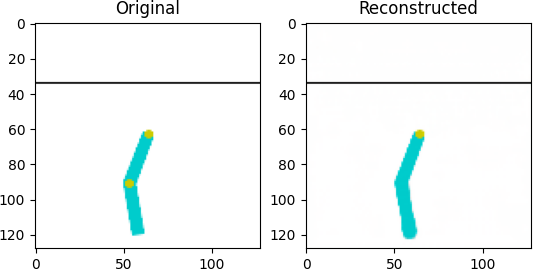
\includegraphics[width=.8\textwidth]{figures/ch5/ae_acrobot.png}
    \caption{Acrobot Reconstruction}
    \label{fig:acrobot_recon}
\end{figure}

\begin{figure}[h]
    \centering
    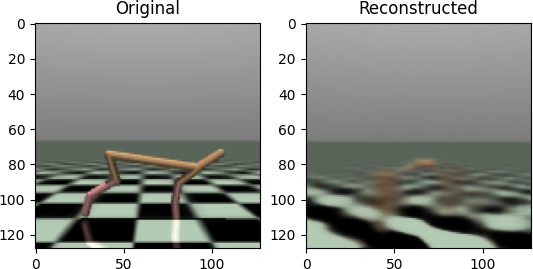
\includegraphics[width=.8\textwidth]{figures/ch5/ae_half_cheetah.png}
    \caption{Half Cheetah Reconstruction}
    \label{fig:half_cheetah_recon}
\end{figure}

\begin{figure}[h]
    \centering
    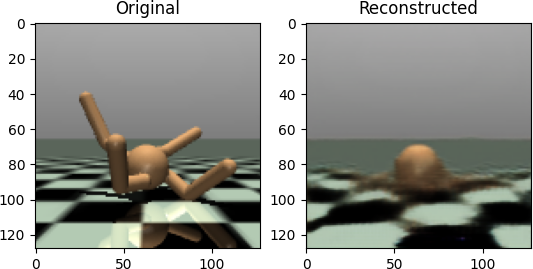
\includegraphics[width=.8\textwidth]{figures/ch5/ae_ant.png}
    \caption{Ant Reconstruction}
    \label{fig:ant_recon}
\end{figure}


These results indicate that while the VAE successfully learned to
encode and reconstruct images from all three environments,
its performance varied significantly across them. The high
reconstruction errors and poor visual quality for Half Cheetah
and Ant suggest that the current VAE architecture may not be
optimal for capturing the complex visual features of these environments.
This limitation, as we will see, could have potentially impacted the effectiveness
of using these learned latent representations in the subsequent reinforcement
learning algorithms, particularly for the more visually complex environments.

\subsection{Reconstruction Loss During Generation}

We measured the Mean Absolute Error (MAE) on a validation set
between the generated counterfactual states and the ground truth
states after the training of WRe-CTDG (comparison between encoded values)
and S-CTDG (comparison between images) frameworks
as shown in Table \ref{tab:mae}.

\begin{table}[h]
\centering
\begin{tabular}{@{}lcc@{}}
    \toprule
    \textbf{Environment} & \textbf{WRe-CTDG MAE} & \textbf{S-CTDG MAE} \\ \midrule
    Acrobot              & 0.25189               & 0.00147             \\
    Half Cheetah         & 0.22064               & 0.03946             \\
    Ant                  & 0.27296               & 0.09391             \\
    Diabetes             & 0.05602               & 0.12710             \\ \bottomrule
    \end{tabular}
\caption{WRe-CTDG and S-CTDG Reconstruction Loss}
\label{tab:mae}
\end{table}

The S-CTDG framework demonstrates superior reconstruction
capabilities across all the image-based environments,
as evidenced by the lower MAE values.
To visually illustrate these reconstruction capabilities, we present a
series of figures comparing original images to their S-CTDG reconstructions
for each environment.

\begin{figure}[h]
    \centering
    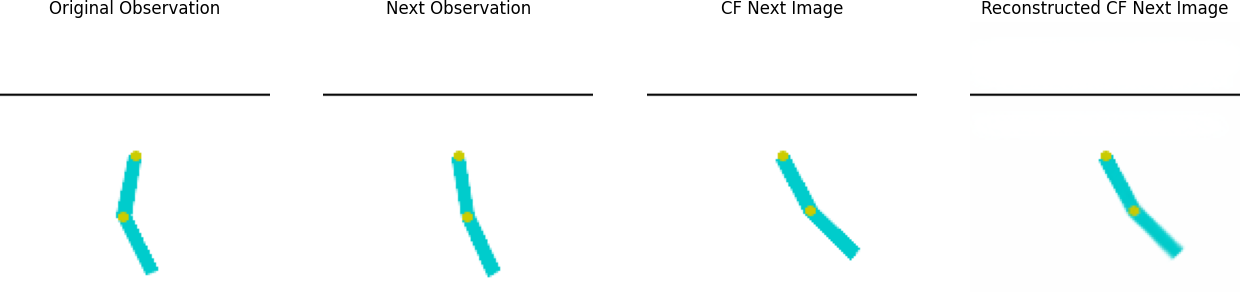
\includegraphics[width=\textwidth]{figures/ch5/e2e_acro.png}
    \caption{S-CTDG results for the Acrobot environment}
    \label{fig:acrobot_recon}
\end{figure}

Figure \ref{fig:acrobot_recon} showcases the S-CTDG reconstruction
for the Acrobot environment. The remarkably low MAE
is reflected in the near-perfect visual fidelity of the reconstructed image,
with virtually no discernible differences from the original.

\begin{figure}[h]
    \centering
    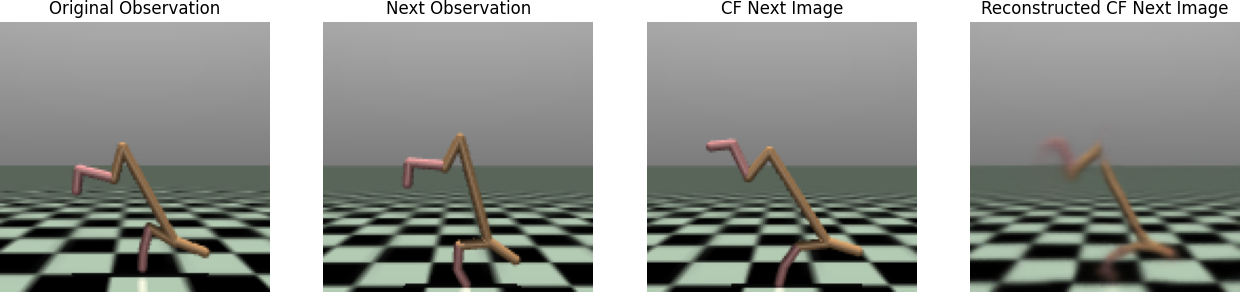
\includegraphics[width=\textwidth]{figures/ch5/e2e_half.png}
    \caption{S-CTDG results for the Half Cheetah environment}
    \label{fig:half_cheetah_recon}
\end{figure}

The Half Cheetah environment reconstruction,
shown in Figure \ref{fig:half_cheetah_recon},
demonstrates the S-CTDG's ability to capture complex articulated structures.
With an MAE of 0.03946, the reconstruction still maintains
the overall structure and positioning of the ant, with some loss of
sharpness in the finer details of the legs and joints.

\begin{figure}[h]
    \centering
    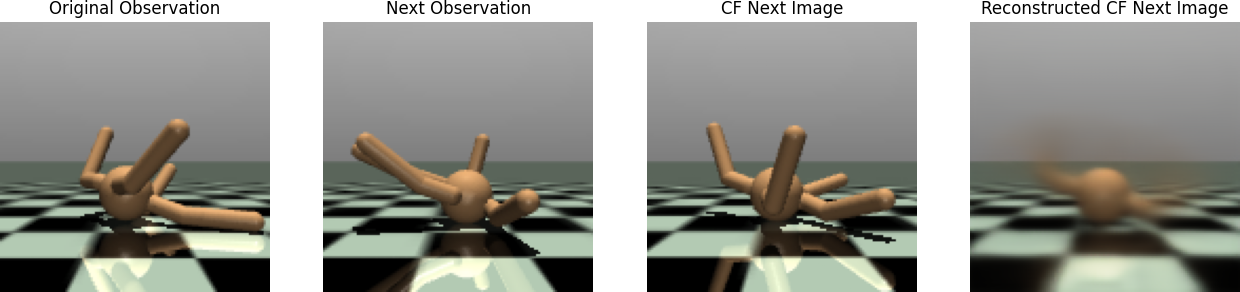
\includegraphics[width=\textwidth]{figures/ch5/e2e_ant.png}
    \caption{S-CTDG results for the Ant environment}
    \label{fig:ant_recon}
\end{figure}

Figure \ref{fig:ant_recon} illustrates the S-CTDG reconstruction
for the Ant environment. Despite the higher MAE of 0.09391 compared
to the previous environments, the reconstruction still captures
the essential features of the ant's body and limbs, albeit with
some loss of detail and sharpness.

For the Diabetes environment, as it doesn't involve image data, we do not provide a visual representation. However, it's worth noting that this is the only environment where WRe-CTDG outperforms S-CTDG in terms of MAE, likely due to the non-visual nature of the data.

\subsection{Reinforcement Learning Performance}

We evaluated the performance of D3QN and TD3 algorithms on both the
original and augmented datasets. The results are presented
in \ref{tab:rl_reward}: the reward value shown is the best reward
over all the evaluation episodes.

\begin{table}[h]
    \centering
    \begin{tabular}{@{}llccc@{}}
        \toprule
        \textbf{Environment} & \textbf{Algorithm} & \textbf{No Aug.} & \textbf{WRe-CTDG Aug.} & \textbf{S-CTDG Aug.} \\ \midrule
        Acrobot              & D3QN               & -57.47           & -53.35                 & -55.90               \\
        Half Cheetah         & TD3                & 8.19             & 74.13                  & 256.09                \\
        Ant                  & TD3                & 27.06            & 25.28                  & 168.54                 \\
        Diabetes             & D3QN               & 0.04             & 0.06                   & 0.12                   \\ \bottomrule
    \end{tabular}
    \caption{Reinforcement Learning Best Reward Value}
    \label{tab:rl_reward}
\end{table}

In Figure \ref{fig:rew_acrobot} we show the reward trends for the
Acrobot environment using D3QN,
in the case of Half Cheetah, we show the reward trends in
Figure \ref{fig:rew_cheetah},
the trends of reward values for the Ant environment
are shown in Figures \ref{fig:rew_ant} and,
at last, the reward trends for the Diabetes environment are shown in
Figures \ref{fig:rew_diabetes}

\begin{figure}[H]
    \centering
    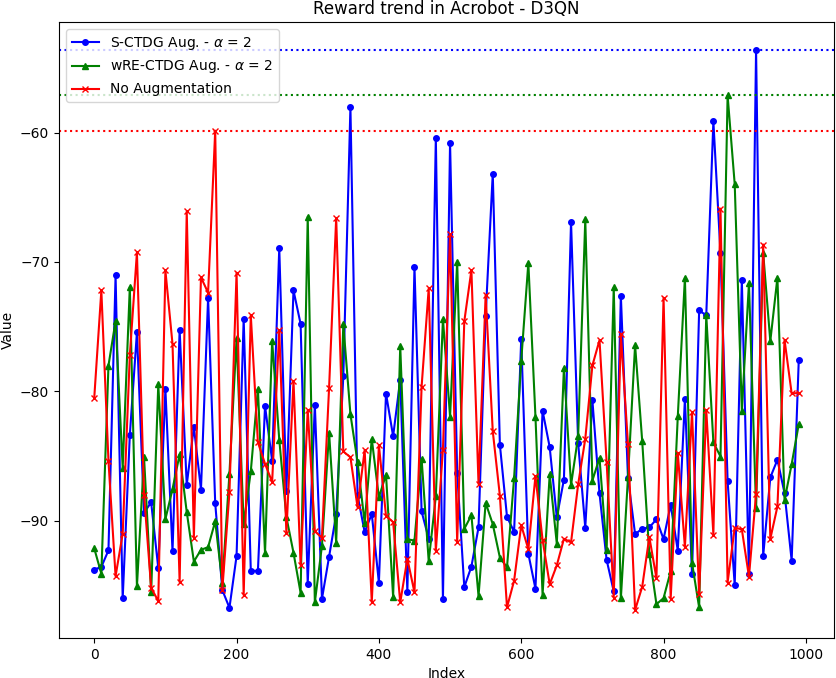
\includegraphics[width=.8\textwidth]{figures/ch5/rew_acrobot.png}
    \caption{Acrobot Reward Trends}
    \label{fig:rew_acrobot}
\end{figure}

\begin{figure}[H]
    \centering
    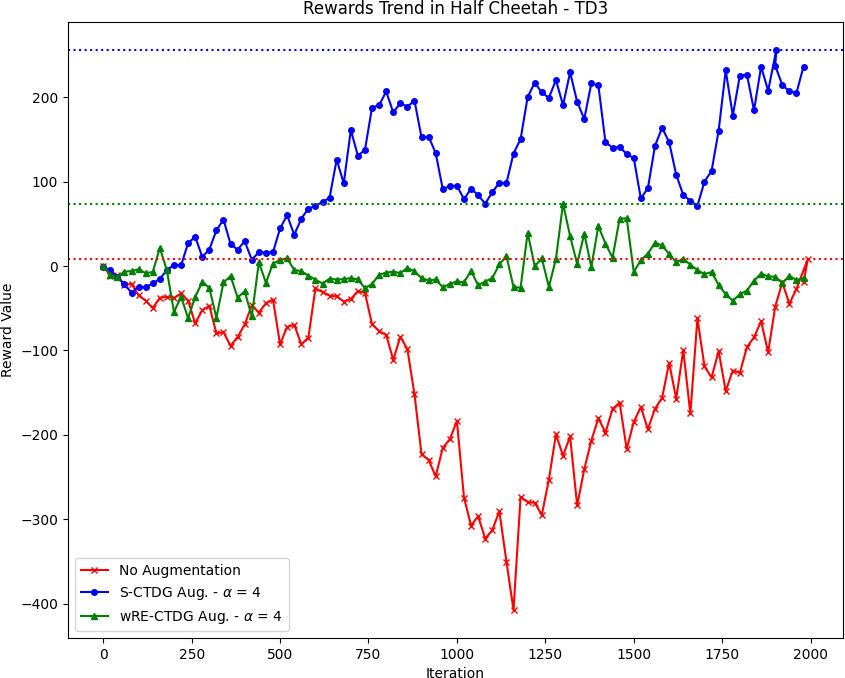
\includegraphics[width=.8\textwidth]{figures/ch5/rew_halfcheetah.png}
    \caption{Half Cheetah Reward Trends}
    \label{fig:rew_cheetah}
\end{figure}

\begin{figure}[H]
    \centering
    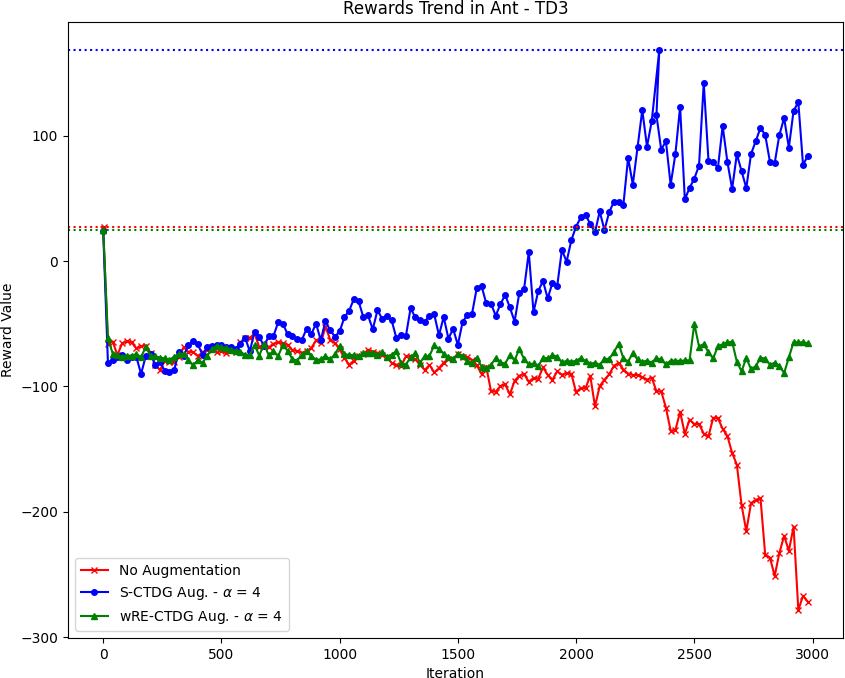
\includegraphics[width=.8\textwidth]{figures/ch5/rew_ant.png}
    \caption{Ant Reward Trends}
    \label{fig:rew_ant}
\end{figure}

\begin{figure}[H]
    \centering
    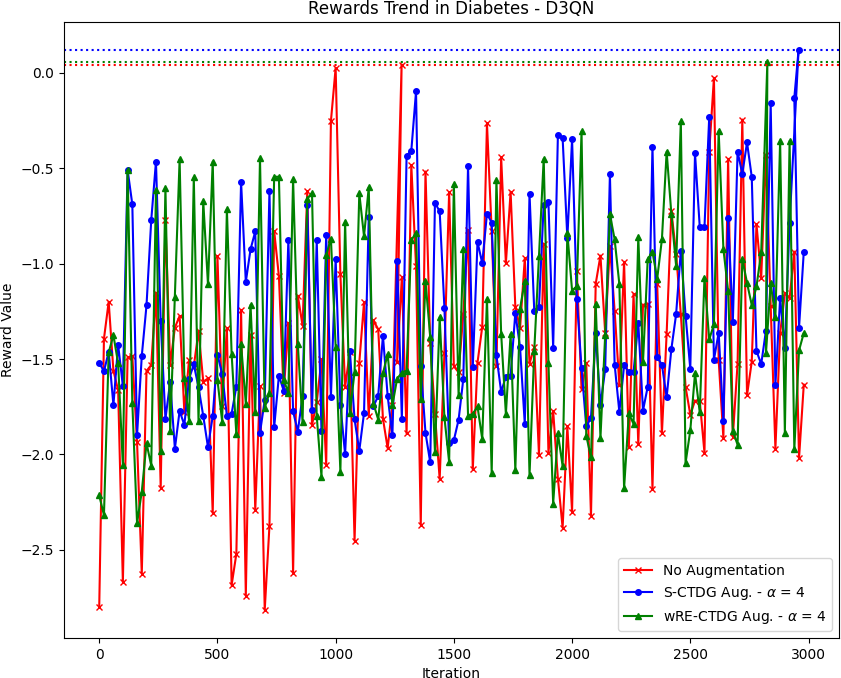
\includegraphics[width=.8\textwidth]{figures/ch5/rew_diabetes.png}
    \caption{Diabetes Reward Trends}
    \label{fig:rew_diabetes}
\end{figure}

\section{Discussion and Analysis of Results}

These findings underscore the potential of counterfactual data generation,
especially S-CTDG, in enhancing the performance of reinforcement learning
algorithms across a variety of tasks and environments.

However, it is important to note that the effectiveness of S-CTDG
comes with significant prerequisites and limitations:
\begin{enumerate}
    \item \textbf{Prior knowledge of system noise:} S-CTDG requires prior
    knowledge of the noise affecting the system.
    This assumption may not always hold in real-world scenarios,
    where the exact nature and distribution of noise might be
    unknown or difficult to model accurately.
    \item \textbf{Ability to perform counterfactual actions:} The S-CTDG
    method necessitates the ability to perform counterfactual actions during
    the data collection process. This requirement can be challenging or
    even impossible to meet in certain environments, particularly in
    real-world applications where data collection might be constrained
    by physical limitations, safety concerns, or ethical considerations.
\end{enumerate}
These constraints highlight an essential trade-off: while S-CTDG
demonstrates superior performance in our experiments,
its applicability may be limited to scenarios where we have
detailed knowledge of the system dynamics and full control over
the data collection process. In contrast, methods like WRe-CTDG,
while generally less effective, may be more broadly applicable as
they don't impose such strict requirements on the data collection
process or prior knowledge of the system.

\chapter{Conclusion}

\section{Summary of Findings}

This thesis has explored novel approaches to address the challenges
of data scarcity and noisy datasets in machine learning, with a specific
focus on offline Deep Reinforcement Learning scenarios.
We introduced two frameworks for counterfactual data generation:
the Wasserstein Reward-enhanced CounTerfactual Data Generation (WRe-CTDG)
and the Supervised CounTerfactual Data Generation (S-CTDG).

Our experimental results demonstrated the efficacy of these
frameworks across various environments and highlight the potential
of counterfactual data generation in enhancing the performance of
offline reinforcement learning algorithms
in across diverse tasks and systems.

\section{Implications and Contributions}

The findings of this research have several important implications:
\begin{itemize}
    \item \textbf{Improved Data Utilization}: Our frameworks demonstrate
    that it's possible to extract more value from existing datasets
    through sophisticated augmentation techniques, potentially 
    reducing the need for extensive data collection.
    \item \textbf{Enhanced Model Performance}: The significant improvements
    in reward values, especially in complex environments
    like Half Cheetah and Ant, suggest that our methods can lead
    to more robust and effective reinforcement learning models.
    \item \textbf{Enhancing Explainability in Reinforcement Learning}: 
    By incorporating causal inference techniques, our work contributes to improving the interpretability and explainability of reinforcement learning models.
    \item \textbf{Applicability to Diverse Domains}: The effectiveness of
    our methods across both robotic simulations and healthcare
    scenarios indicates their potential broad applicability.
\end{itemize}

\section{Limitations}

Despite the promising results, it's important to acknowledge the
limitations of our approach:
\begin{itemize}
    \item \textbf{Prior Knowledge Requirement}: S-CTDG, while
    highly effective, requires prior knowledge of the system
    noise and the ability to perform counterfactual actions
    during data collection. This may limit its applicability
    in some real-world scenarios.
    \item \textbf{Computational Complexity}: The training of the models and
    generation of
    counterfactual data, especially in complex environments,
    can be computationally intensive.
    \item \textbf{Generalization to Other Domains}: While our
    methods showed success in the tested environments, their
    effectiveness in other domains or more complex real-world
    scenarios remains to be fully explored.
\end{itemize}

\section{Future Research Directions}

Based on our findings and identified limitations,
several avenues for future research emerge:
\begin{itemize}
    \item \textbf{Relaxing Prior Knowledge Requirements}: Investigating
    methods to reduce the dependence on detailed prior knowledge of
    system dynamics could broaden the applicability of S-CTDG.
    \item \textbf{Scaling to More Complex Environments}: Exploring
    the effectiveness of these frameworks in increasingly complex
    and realistic environments would be valuable.
    \item \textbf{Real-World Applications}: Applying these
    techniques to real-world offline reinforcement learning problems
    to validate their practical utility.
    \item \textbf{Exploring Advanced ML Architectures}:
    Investigating the integration of state-of-the-art machine
    learning frameworks and structures, such as transformers
    (introduced in \cite{vaswani2023attentionneed})
    and diffusion models
    (presented in \cite{sohldickstein2015deepunsupervisedlearningusing}),
    into our counterfactual data generation approaches,
    for instance:
    \begin{itemize}
        \item \textbf{Transformer}-based models, could improve the
        capture of long-range dependencies in sequential data,
        potentially leading to more coherent and realistic
        counterfactual trajectories.
        \item \textbf{Diffusion models} might offer a new approach
        to generating high-quality counterfactual images, particularly
        in visually complex environments like robotics simulations.
    \end{itemize}
\end{itemize}

In conclusion, this thesis has demonstrated the potential of causal
inference-based counterfactual data generation in addressing the challenge
of data scarcity in offline reinforcement learning.
While there are limitations to be addressed, the promising results
open up exciting possibilities for future research and applications in
this rapidly evolving field.

\appendix

%\include{chapters/AppendiceA}

\nocite{folco}

\bibliographystyle{apalike}
\bibliography{chapters/Bibliografia.bib}

\end{document}
% -----------------------------------------------------------------
